\documentclass[12pt,openany,oneside,a4paper,english,brazil]{abntbibifsemgjf}
\usepackage{lmodern}						
\usepackage[T1]{fontenc}		
\usepackage[utf8]{inputenc}	
\usepackage{lastpage}			
\usepackage{indentfirst}		
\usepackage{color}
\usepackage{graphics}		
\usepackage{graphicx}			
\usepackage{microtype} 			
\usepackage{amsmath}
\usepackage{psfrag}
\usepackage{amsfonts}
\usepackage{amssymb}
\usepackage{tabularx}
\usepackage{lscape}
\usepackage{rotating}
\usepackage{multirow}
\usepackage{tikz}
\usepackage{physics}
\usepackage{pgfplots}
\usepackage{pgfplotstable}
%\usepackage[subpreambles=true]{standalone}
%\usepackage{active}
%\usepackage{tightpage}
%\usepackage{pdftex}
\usetikzlibrary{matrix,chains,arrows,shapes.multipart,automata,calc,fit,tikzmark,trees,shapes}
%\usepackage{cite}
\usepackage[caption=false,font=footnotesize]{subfig}
\usepackage[printonlyused]{acronym}
\usepackage[alf]{abntex2cite}	% Citações padrão ABNT



%% -----------------------------------------------------------------------------
\titulo{Compara\c{c}\~ao de t\'ecnicas de aprendizagem de m\'aquina e processamento de sinal para interfaces cerebrais} %%Por exemplo, Titulo da tese
% \subtitulo{: subtítulo do trabalho}  %% Retirar o primeiro ``%'' desta linha se for utilizar subtitulo. Deixar os dois pontos antes, em ``: subtítulo'' . 

\autor{Otto Luiz Andrade Glass}

\autorR{Glass, Otto Luiz Andrade Glass} %%Colocar o sobrenome do autor antes do primeiro nome do autor, separados por ,

\local{Juiz de Fora}

\data{2020} %%Alterar o ano se precisar

\orientador[Orientador:]{Thiago da Silva Castro} %%Se precisar, troque [Orientador:] por [Orientadora:]
%\coorientador[Coorientador:]{Nome do coorientador} %% Retirar o primeiro ``%'' desta linha se tiver coorientador. Se precisar, troque por [Cooorientadora:]. 

\instituicao{Instituto Federal de Educação, Ciência e Tecnologia do Sudeste de Minas Gerais}

\faculdade{\textit{Campus} Juiz de Fora}

\programa{Engenharia Mecatrônica}

\objeto{Trabalho de Conclusão de Curso}

\natureza{Trabalho de Conclusão de Curso apresentado ao \textit{Campus} Juiz de Fora do Instituo Federal de Educação, Ciência e Tecnologia do Sudeste de Minas Gerais como requisito parcial para obten\c{c}\~ao do grau de Bacharel em Engenharia Mecatrônica.} 

%% Abaixo, prencher com os dados da parte final da ficha catalografica

\autorRR{GLASS, Otto Luiz Andrade} %O ultimo sobrenome deve aparecer primeiro e com todas as letras em maiúsculo.

\finalcatalog{1. Interface Cerebral. 2. Aprendizagem de Maquinas. 3. Ondas Mu. I. Instituto Federal do Sudeste de Minas Gerais. II. T\'itulo.} %% Aqui fica 
% escrito a palavra ``Título'' mesmo, nao o do trabalho. Se tiver coorientador, os dados ficam depois dos dados 
%% do orientador (II. Sobrenome, Nome do coorientador, coorient.) e antes de ``II. Título'', o qual passa a ``III. Título''.



\setlength{\parindent}{1.3cm}
\setlength{\parskip}{0.2cm}  
\setlength\afterchapskip{12pt}  

\hyphenation{tes-te Mecatrônica}

\begin{document}

%% ELEMENTOS PRE-TEXTUAIS
%% Capa
\inserecapa				
%% Folha de rosto
\inserefolhaderosto
%% Ficha catalografica.
\inserecatalog  
%% Folha de aprovacao
\begin{folhadeaprovacao}

  \begin{center}
    {\chapterfont \bfseries \insereautor}

    \vfill
    \begin{center}
      {\chapterfont\bfseries\inseretitulo \inseresubtitulo}
    \end{center}
    \vfill
    
    \hspace{.45\textwidth}
    \begin{minipage}{.5\textwidth}
        \inserenatureza
    \end{minipage}%
    \vfill
   \end{center}
        
   Aprovada em: DD/MM/AAAA %Inserir data da defesa
   
   \begin{center} BANCA EXAMINADORA \end{center}
  \assinatura{Prof. Dr. \insereorientador \ - Orientador \\ Instituto Federal Sudeste de MG - Campus Juiz de Fora} 
%  \assinatura{Prof. Dr. \inserecoorientador \ - Coorientador \\ Instituição}
  \assinatura{Prof. Dr. Beltrano \\ Instituição} %Replicar o número de vezes que for necessário
  \assinatura{Prof. Dr. Beltrano \\ Instituição}
\end{folhadeaprovacao}
%% Dedicatoria. OPCIONAL. Retirar o ``%'' de cada das 4 linhas abaixo, caso queira.
% \begin{dedicatoria} \vspace*{\fill} \centering \noindent
%   \textit{ Dedico este trabalho ... (opcional)} 
%   \vspace*{\fill}
% \end{dedicatoria}
%% Agradecimentos. OPCIONAL. CASO SEJA BOLSISTA, INSERIR OS DEVIDOS AGRADECIMENTOS A AGÊNCIAS DE FOMENTO, FINANCIADORES, LABORATÓRIOS, ETC.
\begin{agradecimentos}

%De acordo com a Associa\c{c}\~ao Brasileira de Normas T\'ecnicas - 14724 (2011, p. 1) Agradecimentos 
%\'e o ``texto em que o autor faz agradecimentos dirigidos \`aqueles que contribu\'iram de maneira relevante \`a elabora\c{c}\~ao do trabalho.''  

\end{agradecimentos}
%% Epigrafe. OPCIONAL
\begin{epigrafe}
    \vspace*{\fill}
	\begin{flushright}
``Algo só é impossível até que alguém duvide dele e prove o contrário''.\\
(Albert Einstein)
	\end{flushright}
\end{epigrafe}

%% RESUMOS
%% Resumo em Portugu^es. OBRIGATORIO.
\setlength{\absparsep}{18pt} 
\begin{resumo}
	
	O objetivo deste trabalho é  realizar a comparação de vários métodos de aprendizagem de máquina e processamento de sinais cerebrais. Analisando a sua performance. Verificando como estes fatores afetam a qualidade da classificação facilitando o desenvolvimento de uma Interface cerebral baseado em sinais motores.
	\par Os métodos utilizados foram o \ac{SVM} e \ac{ANN}, métodos j\'a tradicionais em aplicações de classificação. O trabalho vai em conjunto com métodos de processamentos de sinais os utilizados no trabalho foram \ac{PMTM} , \ac{PSDp} e \ac{PWelch}.
	
	Palavras-chave:  Interface Cerebral, Aprendizagem de Maquinas, Ondas Mu %finalizadas por ponto e inicializadas por letra maiuscula.
	
\end{resumo}
\begin{resumo}[ABSTRACT]
\begin{otherlanguage*}{english}

The objective of this work is to compare a diverse set of methods of machine learning and signal processing, analyzing the performance. To be able to understand how these factors affect the quality of the classification for a \acs{BCI}.
 The machine learning algorithms used for this work were \ac{SVM} and  \ac{ANN}. The signal processing methods used were \ac{PMTM}, \ac{PSDp} and \ac{PWelch}. The \ac{SVM} with a linear kernel was superior to all other machine learning methods.
 


Palavras-chave: Interface Cerebral, Aprendizagem de Maquinas, Ondas Mu %finalizadas por ponto e inicializadas por letra maiuscula.

Keywords: Brain Computer Interface, Machine Learning, Mu wave 
 \end{otherlanguage*}
\end{resumo}

%% Lista de ilustracoes. OPCIONAL.
\pdfbookmark[0]{\listfigurename}{lof}
\listoffigures*
\cleardoublepage

%% Lista de tabelas. OPCIONAL. 
\pdfbookmark[0]{\listtablename}{lot}
\listoftables*
\cleardoublepage


%\pretextualchapter{teste}
\begin{siglas}
	 \setlength{\parskip}{1ex}
	 \setlength{\itemsep}{1ex}
\acro{ANN}{Redes Neurais Artificiais(\textit{Artificial Neural Networks})}
\acro{ANN-2}{Rede neural artificial com 2 camadas ocultas contendo 20 neur\^onios cada}
\acro{ANN-3}{Rede neural artificial com 3 camadas ocultas contendo 20 neur\^onios cada}
\acro{BCI}{Interface Cerebral(\textit{Brain-Computer Interface})}
\acro{BCIs}{Interfaces Cerebrais(\textit{Brain-Computer Interfaces})}
\acro{BP}{Retropropaga\c{c}\~ao (\textit{Backpropagation})}
\acro{C-SVM}{SVM Gaussiano Grosso}
\acro{CTCC}{Comissão do Trabalho de Conclusão de Curso}
\acro{DFT}{Transformada de Fourier Discreta (\textit{Discrete Fourier Transform})}
\acro{ECG}{Eletrocardiograficos}
\acro{EEG}{Eletroencefalograma}
\acro{EEGs}{Eletroencefalogramas}
\acro{EOG}{Eletrooculograma}
\acro{EPS}{\textit{encapsulated postScript}}
\acro{ERD}{Event Related Desynchronization}
\acro{ERS}{Event Related Synchronization}
\acro{F-SVM}{SVM Gaussiano Fino}
%\acro{k-NN}[k-NN]{k-Vizinhos Pr\'oximos(\textit{k-Nearest Neighbours})}
\acro{ICA}{Ana\'alise de Componentes Independentes (\textit{Independent Component Analysis})}
\acro{LDA}{Linear Discriminant Analysis}
\acro{L-SVM}{SVM Linear}
%\acro{NN}{Nearest Neighbour}
\acro{MLP}{perceptrons de m\'ultiplas camadas(\textit{Multilayer Perceptron})}
\acro{OOP}{Programa\c{c}\~ao Orientada a Objetos (\textit{Object Oriented Programing})}
\acro{PCA}{An\'alise de Componente Principal (\textit{Principal Component Analysis})}
\acro{PDF}{\textit{portable document format}}
\acro{PMTM}{Multitaper Power Spectral density}
\acro{PSD}{Power Spectral Density}
\acro{PSDp}{Periodograma}
\acro{PWelch}{Espectro de Welch}
\acro{SCG}{Scaled Conjugate Gradient}
\acro{SVM}{Support Vector Machine}
\acro{TCC}{Trabalho de Conclusão de Curso}
\end{siglas}

%% Sumario
\pdfbookmark[0]{\contentsname}{toc}
\tableofcontents*
\cleardoublepage
\textual
\pagestyle{simple}   

%% TEXTO DA MONOGRAFIA (ELEMENTOS TEXTUAIS)

\chapter{INTRODUÇÃO}

% Introdução ao assunto
\par 
Desde a descoberta da atividade el\'etrica do c\'erebro  e da inven\c{c}\~ao do \linebreak \ac{EEG}, por Hans Berger em 1924, foram desenvolvidas v\'arias id\'eias de como explorar esse acesso \`a fonte de pensamentos, emo\c{c}\~oes e a\c{c}\~oes humanas \cite{10.3389/fnins.2016.00530}.
\ac{BCIs} s\~ao dispositivos que se comunicam diretamente com os sinais cerebrais e permitem a intera\c{c}\~ao direta entre com o meio ambiente \cite{Rao2010}.
\par 
Inicialmente esse campo foi desenvolvido com um foco na restaura\c{c}\~ao de sentidos e mobilidade de pacientes, hoje em dia tamb\'em existe pesquisa em aplica\c{c}\~oes n\~ao-m\'edicas. Por exemplo, como um meio para verificar o alertid\~ao do usu\'ario executando um processo cri\'tico, um dispositivo para jogos e amplifica\c{c}\~ao f\'isica atrav\'es de exoesqueletos \cite{RAO}\cite{10.3389/fnins.2016.00530}.
\par
Para tanto o objetivo de uma \acs{BCI} \'e identificar e prever mudan\c{c}as induzidas pelo comportamento ou o estado cognitivo no sinal cerebral do usu\'ario \cite{Rao2010}.
\par
Para o desenvolvimento de uma \acs{BCI} normalmente s\~ao implementadas as seguintes etapas, como visto na figura \ref{fig:introduction} \cite{RAO}:
\begin{enumerate}
	\item \textbf{Capta\c{c}\~ao do Sinal cerebral}: Sinais cerebrais podem ser captados usando t\'ecnicas invasivas, semi-invasivas ou n\~ao-invasivas.
	
	\item \textbf{Processamento do Sinal}: Sinais brutos s\~ao processados apo\'s a aquisi\c{c}\~ao e t\'ecnicas de redu\c{c}\~ao de artefatos e extra\c{c}\~ao de caracter\'isticas s\~ao utilizadas.
	
	\item \textbf{Aprendizagem de maquina}: Neste est\'agio se gera o sinal de controle normalmente utilizando-se de algoritmos de aprendizagem de m\'aquina. 
	
	\item \textbf{Feedback sensorial}: O sinal de controle gera uma mudan\c{c}a no ambiente.
	Alguns desses mudan\c{c}as podem ser vistas, ouvidas ou sentidas pelo usu\'ario.
	
	\item \textbf{Processamento de sinais para a estimula\c{c}\~ao}: Antes de estimular uma regi\~ao particular no c\'erebro \'e importante sintetizar um padr\~ao de atividade que assemelha a atividade normalmente associada \`aquela regi\~ao. 
	\item \textbf{Estimula\c{c}\~ao cerebral}: O padr\~ao de estimula\c{c}\~ao da etapa anterior \'e utilizada em conjunto com uma t\'ecnica de estimula\c{c}\~ao invasiva ou n\~ao-invasiva para estimular o c\'erebro. 
\end{enumerate}
\par
Durante o desenvolvimento de interfaces cerebrais n\~ao-invasivas utilizando-se do \ac{EEG} encontram-se dois obst\'aculos principais: O fato do sinal ser n\~ao estacion\'ario e sua variabilidade inerente \cite{Rao2010}.
Dados do mesmo paradigma experimental mas de sess\~oes diferentes provavelmente exibir\~ao diferen\c{c}as devido a, por exemplo, ligeiras mudan\c{c}as nas posi\c{c}\~oes dos eletrodos ou mudan\c{c}as nas propriedades eletromec\^anicas eletrodos tal como sua imped\^ancia \cite{Rao2010}.
Al\'em disto, a superposi\c{c}\~ao ruidosa e n\~ao linear da atividade das popula\c{c}\~oes medidas no couro cabeludo podem mascarar os padr\~oes neurais e dificultar sua detec\c{c}\~ao \cite{Rao2010}.
Devido a esses fatores, t\'ecnicas de processamento de sinal estat\'isticas e de aprendizagem de maquina tem uma import\^ancia fundamental durante o processo de reconhecimento de padr\~oes \ac{EEG} e traduzi-los para um sinal de controle \cite{Rao2010}.

\begin{figure}[h!]
	\label{fig:introduction}
	\caption{Est\'agios de uma interface cerebral \cite{Rao2010}}
	\centering
	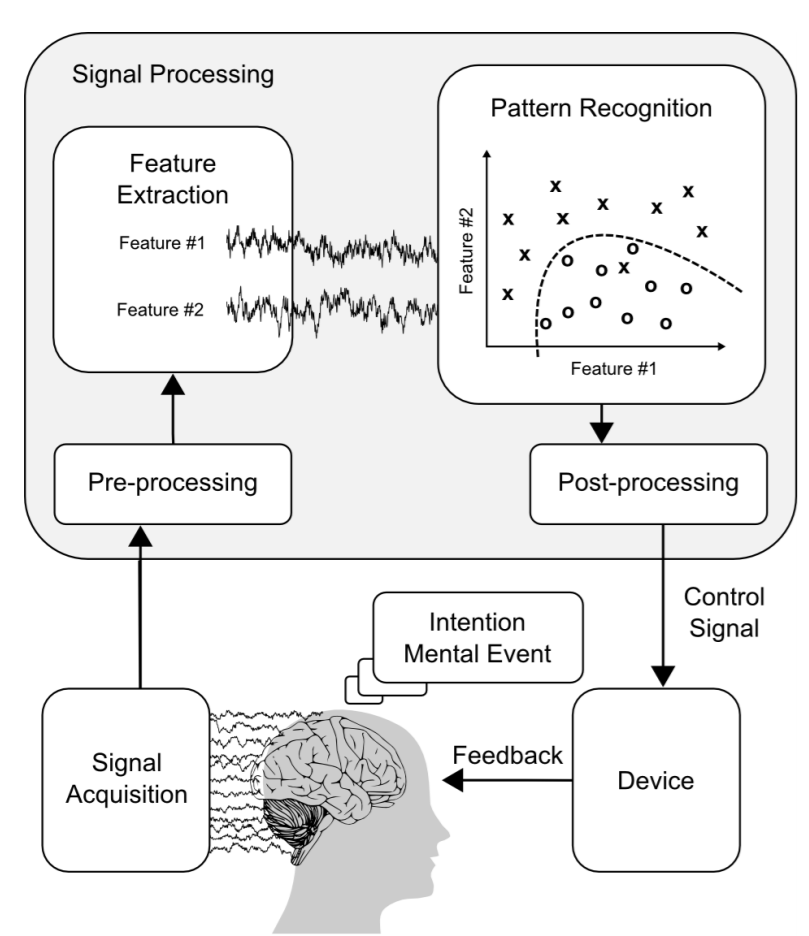
\includegraphics[scale=0.45]{./figuras/bci-stages}
\end{figure}

\section{Objetivo}
%Objetivo Principal
O objetivo principal deste  \ac{TCC} \'e realizar a comparação de m\'etodos de aprendizagem de m\'aquina e processamento de sinais cerebrais para melhor entender como estes fatores afetam a qualidade da classifica\c{c}\~ao permitindo o desenvolvimento de uma \acs{BCI} mais precisa.
\par 
Considerando estes fatores neste trabalho foram explorados e comparados m\'etodos de aprendizagem de m\'aquina tais como redes neurais e SVMs (kernel linear e gaussiano). Tamb\'em foram comparados m\'etodos estimativa de espectro (PMTM, Welch e periodograma) com diferentes configura\c{c}\~oes de comprimento e sobreposi\c{c}\~ao entre as janelas amostradas.
%Objetivo Secundários
Para fazer isto foi nescess\'ario obter as amostras de eletroencefalograma para a classifica\c{c}\~ao;
desenvolver o framework para realizar as compara\c{c}\~oes; fazer a an\'alise dos resultados.
%quatro objetivos secundarios


%



\chapter{Metodologia} \label{label_revisao_bib}
\section{Eletroencefalograma (EEG)}
\subsection{Caracter\'isticas e Sistemas de Medi\c{c}\~ao}
\par
O \ac{EEG} \'e uma das t\'ecnicas n\~ao invasivas mais populares para o desenvolvimento de \ac{BCIs} devido \`a sua alta resolu\c{c}\~ao temporal, baixo custo e por ser de f\'acil instala\c{c}\~ao \cite{RAO}.
\par
Sinais \ac{EEG}, coletados da superf\'icie do couro cabeludo s\~ao flutua\c{c}\~oes de pot\^enciais el\'etricos que refletem a atividade no c\'erebro  principalmente no c\'ortex cerebral abaixo da superf\'cie do couro cabeludo \cite{Vidal77}.
%\par
%O \ac{EEG} consiste em posicionar eletrodos no couro cabeludo.
%Sinais de \ac{EEG} refletem  o somat\'orio de potenciais p\'os-sin\'apticos de milhares de neur\^onios orientados radialmente ao couro cabeludo.
Correntes origin\'arias de regi\~oes mais profundas n\~ao s\~ao detectadas devido ao fato de que campos el\'etricos decaem com o quadrado da dist\^ancia de sua origem.
Portanto, o \ac{EEG} predominantemente captura a atividade no c\'ortex cerebral, cujo o arranjo colunar de neur\^onios e proximidade ao cr\^anio favorecem a sua captura \cite{RAO}.
\par
O padrão internacional sistema 10-20 é tipicamente utilizado para a gravação de \ac{EEG}. Nesse sistema 21 eletrodos são posicionados na superfície do couro cabeludo.
O posicionamento é determinado da seguinte maneira: Os pontos de referência são o n\'asion, que está localizado acima do nariz no nível dos olhos e o ínion que é o ressalto ossudo na base da cr\^anio na linha central do traseiro da cabeça. A partir desses pontos, o perímetro da c é medido dividindo nos planos transverso e mediano. Os locais dos eletrodos podem ser determinadas dividindo esses perímetros em intervalos de 10\% e 20\%. Três outros eletrodos são posicionados em ambos os lados equidistantes dos pontos vizinhos como mostrado na figura \ref{fig:10-20}. \cite{EEGPrinciple}
\begin{figure}[!ht]
	\begin{center}
		\caption{Posi\c{c}\~oes do sistema 10-20 sobre um cr\^anio. Obtido em \cite{EEGPrinciple} }		
		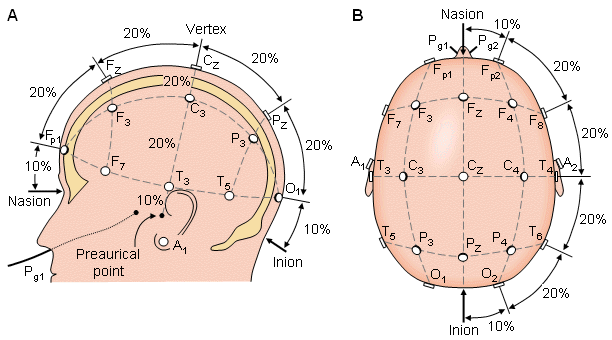
\includegraphics[scale=1]{./figuras/10-20_cranio}
		\label{fig:10-20}
	\end{center}
\end{figure}
\par
Eletrodos bipolares e monopolares podem ser utilizados para a medição do \ac{EEG} (fig. \ref{fig:bipolar-vs-monopolar}).
 No primeiro método é medido a diferença entre um par de eletrodos (fig. \ref{fig:bipolar-vs-monopolar}-A).
 No método posterior o potencial de cada eletrodo é comparado a um eletrodo neutro ou \`a m\'edia de todos os eletrodos como pode ser observado na figura \ref{fig:bipolar-vs-monopolar}-B \cite{EEGPrinciple}.
\begin{figure}[!ht]
	\begin{center}
		\caption{Compara\c{c}\~ao do sinal Monopolar (B) vs o Bipolar (A). Obtido em \cite{EEGPrinciple} }		
		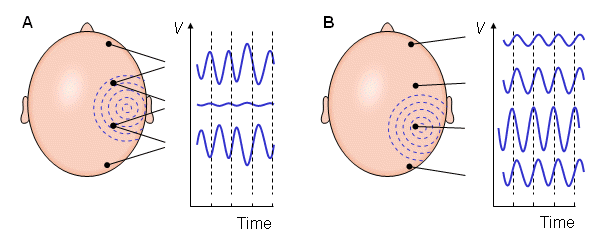
\includegraphics[scale=1]{./figuras/Bipolar-vs-Monopolar}
		\label{fig:bipolar-vs-monopolar}
	\end{center}
\end{figure}
\clearpage
\subsection{Ritmo $\mu$}
No \ac{EEG}, em humanos a regi\~ao pr\'oxima ao c\'ortex motor exibe tipicamente um sinal, de 10$\mu V$-50$\mu V$ e na banda de frequ\^encia de aproximadamente 8-12Hz, enquanto n\~ao est\'a produzindo atividade motora, este sinal \'e denominado de ritmo  $\mu$ (figura \ref{fig:Mu}).
Movimento real ou imagin\'ario \'e normalmente acompanhada de uma redu\c{c}\~ao no ritmo $\mu$ no lado do c\'erebro oposto ao movimento como pode ser visto na figura \ref{fig:mu-left-vs-right}.
Est\'a redu\c{c}\~ao de atividade \'e referida como \ac{ERD} por \cite{EOG2006} e como \ac{ERS} por \cite{Vidal77}.
\cite{BCI2000} \cite{RAO}
\begin{figure}[!ht]
	\begin{center}
		\caption{(A,B) distribui\c{c}\~ao topogr\'afica no couro cabeludo da diferen\c{c}a calculada do movimento da m\~ao direita (A) real e (B) imagin\'ario de uma pessoa vs ela relaxada com o sinal numa banda 10,5-13,5Hz. (C) O espectro  para um outro sujeito em C3 comparando o estado relaxado (linha cortada) vs imagina\c{c}\~ao motora e (D) o espectro $r^2$ para a imagina\c{c}\~ao motora vs o estado relaxado deste sujeito \cite{BCI2000}}
		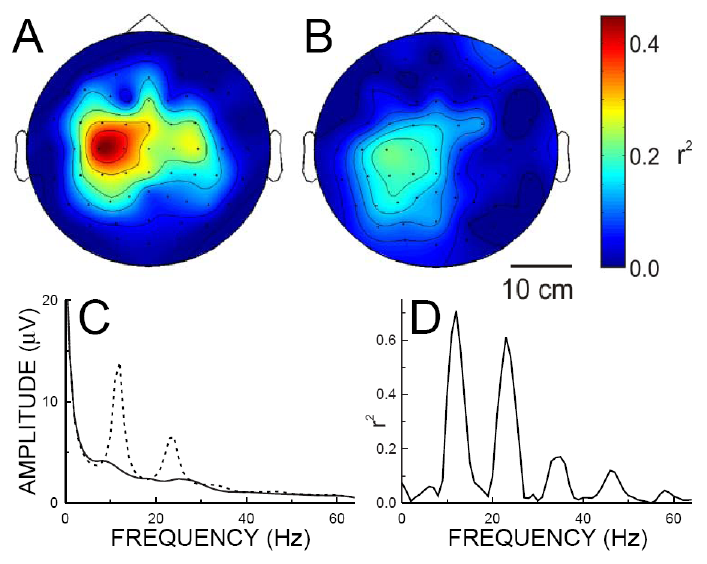
\includegraphics[scale=0.35]{./figuras/ERDmu}
		\label{fig:Mu}
	\end{center}
\end{figure}
\begin{figure}[!ht]
	\begin{center}
		\caption{O Efeito da imagina\c{c}\~ao motora esquerda vs direita no ritimo $\mu$ tal como captado pelos eletrodos em C3 (lado esquerdo) e C4 (lado direito) \cite{Qin2004}} 		
		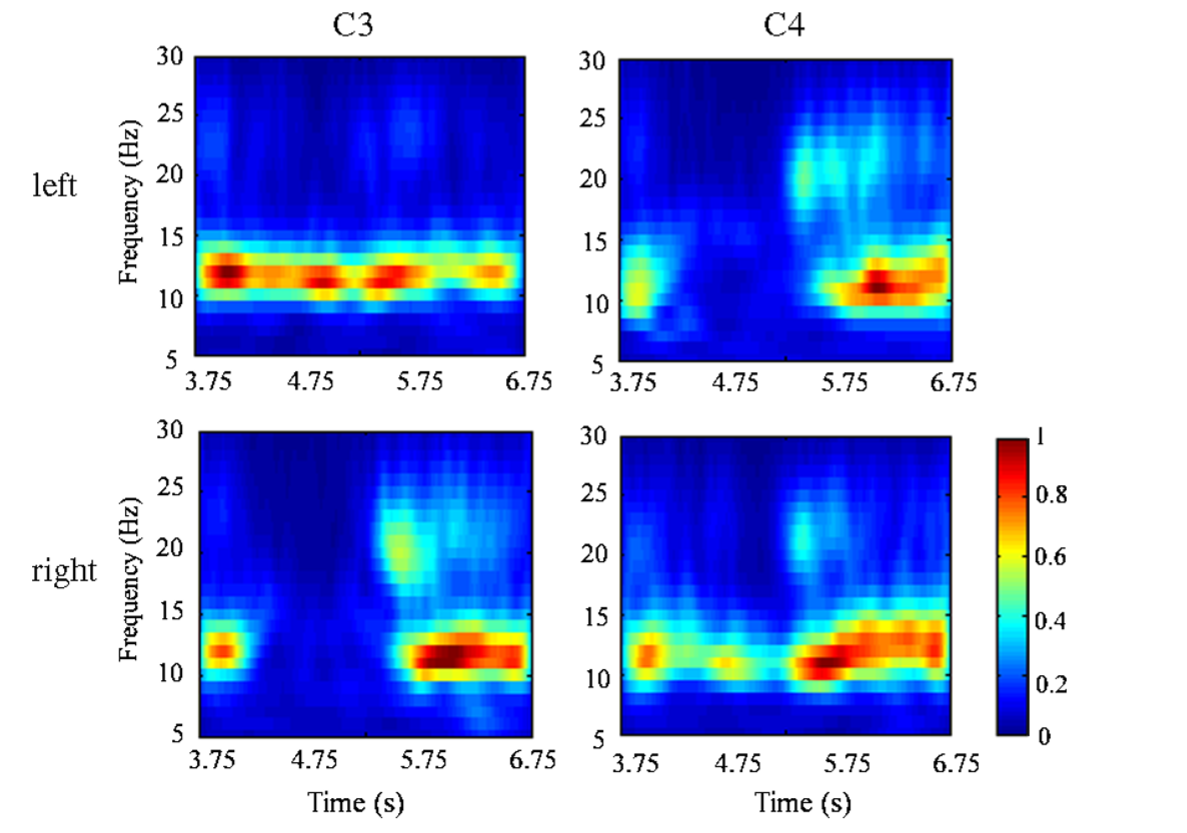
\includegraphics[scale=0.45]{./figuras/mu-left-vs-right}
		\label{fig:mu-left-vs-right}
	\end{center}
\end{figure}
\subsection{Redu\c{c}\~ao de Artefatos}
\par
Artefatos s\~ao flutua\c{c}\~oes pot\^encias de origem n\~ao neural. Essas incluem pot\^encias eletro oculares, musculares (do pesco\c{c}o, couro cabeludo e do rosto), \ac{ECG} al\'em de fontes externas como o ru\'ido de rede el\'etrica 50/60Hz  \cite{Vidal77} \cite{RAO}.
\par
Artefatos no geral e especificamente no \ac{EOG} s\~ao uma grande fonte de ru\'idos em grava\c{c}\~oes de \ac{EEGs}.
Pode-se assumir que toda grava\c{c}\~ao \ac{EEG} est\'a contaminada com artefatos \ac{EOG}, pois movimentos oculares s\~ao dif\'iceis de suprimir por per\'iodos prolongados.
Por exemplo um estudo em \ac{EEG} do sono 9.1\% do total grava\c{c}\~ao estava contaminada com artefatos \ac{EOG} \cite{EOG2006}.
\par
A origem do \ac{EOG} \'e devido \`a atividade el\'etrica do olho que \'e propagada pelo corpo e pode ser gravado pelo corpo em sua superf\'icie.
Artefatos \ac{EOG} s\~ao causados pelos movimentos do dipolo retinal e das p\'alpebras.
Um modelo simplificado assume um dipolo el\'etrico dentro dos olhos.
A dire\c{c}\~ao do dipolo \'e alinhada com a linha de vis\~ao e a amplitude do dipolo \'e determinada pela quantidade de luz atingindo a retina.
Na maioria dos casos ambos olhos est\~ao na mesma linha de vis\~ao e observam a mesma lumin\^ancia. Portanto ambos os dipolos s\~ao paralelos e altamente correlacionados.
Por conta disso o \ac{EOG} pode ser modelado por um \'unico dipolo. 
Devido aos efeitos da condu\c{c}\~ao de volume, o \ac{EOG} e \ac{EEG} s\~ao propagados pela superf\'icie da cabe\c{c}a onde a superposi\c{c}\~ao de ambos \'e gravado.
Os pesos dos componentes dessas superposi\c{c}\~ao s\~ao determinados pelas rela\c{c}\~oes espaciais e propriedades el\'etricas dos tecidos entre as fontes e os eletrodos.
Essas propriedades n\~ao se alteram durante uma grava\c{c}\~ao com a exce\c{c}\~ao do movimento das p\'alpebras que alteram a geometria do tecido proximo delas.
Por\'em esse efeito do movimento das p\'alpebras pode ser modelado como uma componente radial do \ac{EOG}, portanto os pesos dos componentes na superposi\c{c}\~ao podem ser considerados est\'aticos \cite{EOG2006}.
\par
Para a redu\c{c}\~ao de artefatos \ac{EOG} existem v\'arias t\'ecnicas dentre elas \ac{PCA}, \ac{ICA} e regress\~ao linear.
A seguir ser\'a descrito o m\'etodo discutido em \cite{EOG2006} que \'e uma regress\~ao linear.
\par
O seguinte modelo linear \'e assumido contendo 3 componentes espaciais (horizontal, vertical e radial) de \ac{EOG}: 
\begin{equation}
Y(t,ch)=S(t,ch)+[EOG1(t),EOG2(t),EOG3(t)]
\cdotp
[b_1(ch),b_2(ch),b_3(ch)]^T
\end{equation}
Onde $Y(t,ch)$ \'e o valor gravado de cada canal ch num tempo t, S \'e a fonte do sinal sem contami\c{c}\~ao de artefatos, EOG123 indicam a fonte de ruido $U$ das 3 componentes espaciais do EOG e $b(ch)$ indicam os pesos dos componentes EOG no canal \ac{EEG} ch.
Para podermos obter o sinal corrigido a fonte de ru\'idos $U$ e os pesos $b$ tem que serem conhecidos.
O \ac{EOG} pode ser gravado num canal separado.
Para obter $b$  tem que se assumir de que o sinal $S$ e o ru\'ido $U$ s\~ao linearmente independentes, assumindo isso.
\begin{equation}
S=Y-U \cdotp b
\end{equation}
\begin{equation}
<U^T S>=<U^T Y> - <U^T U>b
\end{equation}
onde $<U^T S>=0$ resultando em
\begin{equation}
b=<U^T U>^{-1} <U^T Y>
\end{equation}
permitindo que $S$ seja calculado.
\clearpage
\section{Redes Neurais}
\par
Redes neurais baseadas em Backpropagation tem se mostrado bem sucedido em uma alta variedade de tarefas de classifica\c{c}\~ao , incluindo a classifica\c{c}\~ao de dados de \ac{BCI}.
Apesar de serem poderosas tais redes neurais frequentemente sofrem de um problema de \textit{overfitting} aos dados de treinamento, resultando numa genereliza\c{c}\~ao fraca.
Por consequ\^encia disso \ac{SVM}s s\~ao tipicamente favorecidas sobre \ac{ANN} como o algor\'itmo de escolha em muitas \ac{BCI} \cite{RAO}. Mas o seu entendimento ainda \'e importante, pois novas t\'ecnicas est\~ao sendo derivadas de \ac{ANN} tal como Redes Neurais Convolucionais \cite{nigam2020}. 
\par
\ac{ANN} s\~ao inspiradas pela sua contraparte na biologia e procuram reproduzir algumas das capacidades adaptativas de redes neurais no c\'erebro em classificar dados de entrada de maneira robusta \cite{Haykin2008}. 

\subsection{Neur\^onios Artificiais}
O modelo de um neur\^onio que forma as \ac{ANN} \'e mostrado na figura \ref{fig:neuronioartificial} e consiste em 3 partes:
\begin{enumerate}
	\item Um conjunto de sin\'apses (conex\~oes) cada uma caracterizada por um peso $w_{l\left< k,j \right> }$ onde $k$ \'e o \'indice do neur\^onio na camada $l$ e $j$ \'e o \'indice do n\'o de origem na camada anterior ($l-1$).
	\item Um somador para somar todos os sinais de entrada multiplicado pelo seu \textbf{peso} $w_{l\left< k,j \right> }$ e o valor do \textbf{bias} $b_{(l,k)}$.
	\item Uma fun\c{c}\~ao de ativa\c{c}\~ao $\varphi(s)$ para restringir a amplitude da sa\'ida de um neur\^onio. tipicamente a amplitude da saida de um neur\^onio varia de [0,1] ou [-1,1].
\end{enumerate}
Este modelo tamb\'em pode ser representado por esse par de equa\c{c}\~oes:
\begin{equation}
s=\sum_{j=1}^{n} w_{l\left< k,j \right> } x_j
\end{equation}
e
\begin{equation}
y_k=\varphi \left( s+b_{(l,k)} \right) 
\end{equation}
\begin{figure}[!h]
	\begin{center}
		\caption{Diagrama neuronio}		
		\tikzstyle{weightNode}=[draw,rectangle,minimum size=10pt,inner sep=3pt]
\tikzstyle{stateTransition}=[->, thick]
\tikzstyle{biasNode}=[-stealth]
\tikzstyle{nonlinearityNode}=[draw,rectangle,minimum size=25pt, inner sep=2pt]
\begin{tikzpicture}
\node[draw,circle,minimum size=25pt,inner sep=0pt] (x) at (0,0) {$\Sigma$};
\foreach \l [count=\n] in {0,1,2,3,n} {
	\node[weightNode] (w\l) at (-2.2,{1.1*(3-(\n))}) {$ w_{l \left< k ,\l \right>}$};
	\draw[stateTransition] (w\l) to [out=0,in={82.5+\n*32.5}] node [midway, sloped, above=-2] {} (x);
	\node[biasNode] (x\l) at (-3.7,{1.1*(3-(\n))}){$x_\l$};
	\draw[stateTransition,o->] (x\l) -- (w\l);
}
\node[biasNode]  (b)  at (0,2) {$b_{(l,k)}$};
\node[nonlinearityNode] (phi) at (1.75,0) {$\varphi \small{\left(  s \right)  } $};
\draw[stateTransition] (phi) -- (3,0) node [midway,above=-0.1cm] {$y_k$};
\draw[stateTransition,o->] (b) -- (x);
\draw[stateTransition] (x) -- (phi);
\node (dots) at (-3.75, -1.5) {$\vdots$};
\end{tikzpicture}
		\label{fig:neuronioartificial}
	\end{center}	
\end{figure}
\subsection{Tipos de Fun\c{c}\~oes de ativa\c{c}\~ao}
\begin{itemize}
	\item \textbf{Fun\c{c}\~ao Sinal}: \'e uma fun\c{c}\~ao de ativa\c{c}\`ao simples descrita pela equa\c{c}\~ao \ref{eq:sign}.
	\begin{equation}\label{eq:sign}
	\varphi \left( s \right) =\begin{cases}
	1 \text{ se } s > 0\\
	0 \text{ se } s = 0\\
	-1 \text{ se } s < 0
	\end{cases}
	\end{equation}
	Ela \'e uma das fun\c{c}~oes de ativa\c{c}\~ao mais simples e \'e utilizada no perceptron de uma camada, \ac{LDA} e \ac{SVM} entre outros.
	\begin{figure}[!h]
		\begin{center}
			\caption{Fun\c{c}\~ao Sinal}			
			\begin{tikzpicture}[domain=-1.5:1.5,scale=2]
%\draw[very thin,color=gray,step=0.25] (-1.4,-1.4) grid (1.4,1.4);
\draw[loosely dashed,thick](-1.6,-1) -- (+1.6,-1) node[right] {$-1$};
\draw[loosely dashed,thick](-1.6,1) -- (+1.6,1) node[right] {$1$};
\draw[->] (-1.6,0) -- (1.6,0) node[right]{$s$};
\draw[->] (0,-1.6) -- (0,1.6) node[above]{$\varphi \left( s \right) $};
\draw[color=cyan,very thick] (-1.6,-1) -- (-0.015,-1);
\draw[dotted,color=cyan,very thick] (-0.015,-1) -- (0.015,1);
\draw[color=cyan,very thick] (0.015,1) -- (1.6,1);
\end{tikzpicture}
			\label{fig:funcaosinal}
		\end{center}	
	\end{figure}
	\item \textbf{Fun\c{c}\~ao Logi\'stica}
	\'e uma fun\c{c}\~ao do tipo sigm\'oide, cujo gr\'afico tem forma de s, \'e a fun\c{c}\~ao de ativa\c{c}\~ao mais comum para o uso em \ac{ANN}. Ela tem uma amplitude de [0,1] ela \'e dada pela equa\c{c}\~ao \ref{eq:log}.
	\begin{equation}\label{eq:log}
	\varphi \left( s \right) = \frac{1}{1+exp(-a s)}
	\end{equation}
	Ela \'e deriv\'avel e sua derivada \'e extremamente simples e dada por eq. \ref{eq:divlog}
	\begin{equation}\label{eq:divlog} 
	\dv{\varphi \left( s \right)}{s}  = \varphi \left( s \right)\left( 1 -  \varphi \left( s \right) \right)
	\end{equation}	
	\begin{figure}[!ht]
		\begin{center}
			\caption{Fun\c{c}\~ao log\'istica}			
			\begin{tikzpicture}[domain=-1.5:1.5,scale=2]
%\draw[very thin,color=gray,step=0.25] (-1.4,-1.4) grid (1.4,1.4);
\draw[loosely dashed,thick](-1.6,-1) -- (+1.6,-1) node[right] {$-1$};
\draw[loosely dashed,thick](-1.6,1) -- (+1.6,1) node[right] {$1$};
\draw[->] (-1.6,0) -- (1.6,0) node[right]{$s$};
\draw[->] (0,-1.6) -- (0,1.6) node[above]{$\varphi \left( s \right) $};
\draw[very thick,color=cyan] plot (\x,{1/(1+exp(-5*\x))});
\end{tikzpicture}
			\label{fig:funcaologistica}
		\end{center}	
	\end{figure}
	\item \textbf{Fun\c{c}\~ao tangente hiperb\'olica} \'e uma outra fun\c{c}\~ao do tipo sigm\'oide sua amplitude \'e de [-1,1] o fato de ser uma fun\c{c}\~ao impar reduz o numero de itera\c{c}\~oes nescess\'arias se comparado \`a fun\c{c}\~ao log\'istica (mais detalhes sobre isso pode-se encontrar em \cite{Haykin2008} se\c{c}\~ao 4.11). 
	\begin{equation} \label{eq:tanh}
	\varphi \left( s \right)  = tanh(s)
	\end{equation}	
	E sua derivada Eq. \ref{eq:divtanh}.
	\begin{equation}\label{eq:divtanh}
	\dv{\varphi \left( s \right)}{s}  = 1 -  \varphi^2 \left( s \right) 
	\end{equation}	
	\begin{figure}[!h]
		\begin{center}
			\caption{Fun\c{c}\~ao tangente hiperb\'olica}			
			\begin{tikzpicture}[domain=-1.5:1.5,scale=2]
%\draw[very thin,color=gray,step=0.25] (-1.4,-1.4) grid (1.4,1.4);
\draw[loosely dashed,thick](-1.6,-1) -- (+1.6,-1) node[right] {$-1$};
\draw[loosely dashed,thick](-1.6,1) -- (+1.6,1) node[right] {$1$};
\draw[->] (-1.6,0) -- (1.6,0) node[right]{$s$};
\draw[->] (0,-1.6) -- (0,1.6) node[above]{$\varphi \left( s \right) $};
\draw[very thick,color=cyan] plot (\x,{tanh(2*\x)});
\end{tikzpicture}
			\label{fig:funcaotanh}
		\end{center}	
	\end{figure}	
\end{itemize}
\subsection{Perceptron de m\'ultiplas camadas}
\par
As \ac{ANN} chamadas de \ac{MLP} consistem tipicamente de um conjunto de n\'os de entrada que constituem a \textit{camada de entrada}, uma ou mais \textit{camadas ocultas} e uma \textit{camada de sa\'ida} isto pode ser visto na figura \ref{fig:MLP} \cite{Haykin2008}.

\begin{figure}[!h]
	\begin{center}
		\caption{Diagrama de MLP gen\'erico}		
		\tikzset{%
  every neuron/.style={
    circle,
    draw,
    minimum size=1cm
  },
  neuron missing/.style={
    draw=none, 
    scale=2,
    text height=0.333cm,
    execute at begin node=\color{black}$\vdots$
  },
  every input/.style={
  	rectangle,
  	draw,
  	minimum size=0.2cm
  },
  input missing/.style={
	draw=none, 
	scale=2,
	text height=0.333cm,
	execute at begin node=\color{black}$\vdots$
},
}

\begin{tikzpicture}[x=1.5cm, y=1.5cm, >=stealth]

\foreach \m/\l [count=\y] in {1,2,3,4,missing,5}
  \node [every input/.try, input \m/.try] (input-\m) at (0,2.7-\y) {};

\foreach \m [count=\y] in {1,2,missing,3}
  \node [every neuron/.try, neuron \m/.try ] (hidden-\m) at (2,2-\y*1.1) {};

\foreach \m [count=\y] in {1,missing,2}
  \node [every neuron/.try, neuron \m/.try ] (output-\m) at (4,1.5-\y) {};

\foreach \l [count=\i] in {1,2,3,4,n}
  \draw [<-] (input-\i) -- ++(-1,0)
    node [above, midway] {$I_\l$};

\foreach \l [count=\i] in {1,2,n}
  \node [above] at (hidden-\i.north) {$H_\l$};

\foreach \l [count=\i] in {1,n}
  \draw [->] (output-\i) -- ++(1,0)
    node [above, midway] {$O_\l$};

\foreach \i in {1,...,5}
  \foreach \j in {1,...,3}
    \draw [->] (input-\i) -- (hidden-\j);

\foreach \i in {1,...,3}
  \foreach \j in {1,...,2}
    \draw [->] (hidden-\i) -- (output-\j);

\foreach \l [count=\x from 0] in {de entrada, oculta, de sa\'ida}
  \node [align=center, above] at (\x*2,2.3) {camada \\ \l};

\end{tikzpicture}
		\label{fig:MLP}
	\end{center}	
\end{figure}
\par
Um \ac{MLP} tem tr\^es caracter\'isticas distintivas \cite{Haykin2008}:
\begin{enumerate}
	\item 	O modelo de cada neur\^onio inclui uma fun\c{c}\~ao de ativa\c{c}\~ao n\~ao-linear continuamente diferenci\'avel.
	A n\~ao linearidade \'e nescess\'aria pois sem ela a rede pode ser reduzida a uma \'unica camada (a camada de sa\'ida).
	\item  A rede cont\'em uma ou mais camadas de neur\^onios ocultos, que n\~ao fazem parte da entrada ou sa\'ida da rede. 
	\item A rede exibe um alto grau de \textbf{conectividade}, determinado pelas sinapses da rede.
\end{enumerate}
\subsection{Aprendizagem}
Dentre das regras de aprendizagem uma das mais antigas \'e a aprendizagem Hebbiana que simplificada diz \cite{Haykin2008}:
\begin{enumerate}
	\item Quando dois neur\^onios em ambos os lados da sinapse s\~ao ativados ao mesmo tempo o peso da conex\~ao entre eles \'e fortalecido.
	\item Quando dois neur\^onios em ambos lados da sinapse s\~ao ativados de maneira dessincronizada o peso da conex\~ao entre eles \'e enfraquecido.
\end{enumerate}
No caso do \acl{MLP} isto pode ser descrito pela eq. \ref{eq:Hebb} onde $\textbf{w}_n$ \'e o vetor dos pesos e bias da rede na itera\c{c}\~ao $n$.  
\begin{eqnarray}\label{eq:Hebb}
\textbf{w}_{n+1}=\textbf{w}_n+\Delta \textbf{w}_n\\
\textbf{w}=\left(w_{1\left< 1,1 \right> },\dots,w_{1\left< 1,j \right>},b_{\left(1,1 \right)},\dots,w_{L\left< K,J \right>},b_{\left(L,K \right)} \right)
\end{eqnarray}
Para determinar o valor de $\Delta \textbf{w}_n$, uma abordagem \'e escolher um  $\Delta \textbf{w}_n$ que minimize o erro de classifica\c{c}\~ao da rede num conjunto de treinamento. Essa abordagem \'e denominada \textit{aprendizagem por corre\c{c}\~ao de erro} \cite{Haykin2008} e pode ser formulada pela eq. \ref{eq:AprendizagemErro} onde, $\eta$ \'e o tamanho do passo, tamb\'em conhecido como \textit{taxa de aprendizagem}  e $\textbf{p}_n$ \'e um vetor com a dire\c{c}\~ao que minimiza a fun\c{c}\~ao de erro  de clasifica\c{c}\~ao $E(\textbf{w})$.
\begin{equation}\label{eq:AprendizagemErro}
\Delta \textbf{w}_n= \eta \textbf{p}_n
\end{equation}

\subsection{Backpropagation(BP)}

O algoritmo Backpropagation é um algoritmo que lida com os pesos de uma rede de acordo com os erros obtidos em seus neurônios adjacentes.  Ele utiliza um método gradiente como tentativa de minimizar o erro $E_{total}(\textbf{t},\textbf{o})$ entre os valores de saída e os valores alvos. A equação \ref{eq:backpropagation} mostra o principio básico do calculo para o erro, sendo a métrica utilizada em algoritmos b\'asicos o MSE (Erro médio quadrático). Sendo N o número de amostras, $t_n$ é a reposta alvo e $o_n$ é a resposta calculada da rede \cite{Haykin2008}.


\begin{equation}\label{eq:backpropagation}
E_{total}(\textbf{t},\textbf{o})  = \frac{1}{2N} \sum_{n=0}^{N} (t_n - o_n)^2
\end{equation}

Para cada entrada $I_{1}$ e $I_{2}$ e saída $O_{1}$ da Figura \ref{fig:BPNN} teremos:
\begin{itemize}
	\item A propagação das entradas $I_{1}$ e $I_{2}$ pela rede, e computando a saída $O_{1}$ para cada dado de treinamento.
	\item Para a saída $O_{1}$ é calculado então um erro $E_{total}(\textbf{t},\textbf{o})$ que está relacionado \`a sua sa\'ida e o resultado alvo esperado.
	\item A partir disso é calculado os erros dos pesos, utilizando a regra da cadeia, aos neurônios ocultos das camadas internas. Retropropagando o erro desde as camadas de saída até a ultima camada interna (figura \ref{fig:BPNNAmp}).
	\item Após o calculo dos erros de cada neur\^onio, é utilizado um método gradiente para o cálculo das novas sinapses de cada conexão. A equação \ref{eq:bpgradi} mostra um modo de como pode ser atualizado o peso sendo $\Delta w_{ij}$ o peso da conexão entre os neurônios i e j, $\eta$ a Taxa de aprendizado e $E_(w)$ o próprio erro. 
\end{itemize}
\par
Para classifica\c{c}\~ao uma das fun\c{c}\~oes de erro mais utilizadas \'e entropia cruzada.
Ela penaliza fortemente classifica\c{c}\~oes incorretas e \'e dada pela eq. \ref{eq:crossentropy} onde $o_n$ \'e a sa\'ida $n$ da rede e $t_n$ \'e o valor alvo daquela sa\'ida.
\begin{eqnarray}\label{eq:crossentropy}
E_n(t_n,o_n) = \frac{-t_n log(o_n)}{N}\\
E_{total}(\textbf{t},\textbf{o}) = \sum_{n=0}^{N} \frac{-t_n log(o_n)}{N}
\end{eqnarray}
e sua derivada \'e
\begin{equation}\label{eq:divcrossentropy}
\dv{E_n(t_n,o_n)}{o_n} = \frac{-t_n}{o_n N}\\
\end{equation}
\begin{equation}\label{eq:bpgradi}
\Delta w_{ij} = -\eta \frac{\partial E_(w) }{\partial w_{ij}}
\end{equation}


\begin{figure}[!htp]
	\begin{center}
		\caption{Exemplo de NN para calcular o Backpropagation}		
		\tikzset{%
  every neuron/.style={
    circle,
    draw,
    minimum size=1cm
  },
  neuron missing/.style={
    draw=none, 
    scale=2,
    text height=0.333cm,
    execute at begin node=\color{black}$\vdots$
  },
  every input/.style={
  	rectangle,
  	draw,
  	minimum size=0.2cm
  },
  input missing/.style={
	draw=none, 
	scale=2,
	text height=0.333cm,
	execute at begin node=\color{black}$\vdots$
},
}

\begin{tikzpicture}[x=1.5cm, y=1.5cm, >=stealth]

\foreach \m/\l [count=\y] in {1,2}
  \node [every input/.try, input \m/.try] (input-\m) at (0,{1.3-(\y-1)*2}) {};

\foreach \m [count=\y] in {1,2}
  \node [every neuron/.try, neuron \m/.try ] (hidden-\m) at (2,2-\y*1.1) {};

\foreach \m [count=\y] in {1}
  \node [every neuron/.try, neuron \m/.try ] (output-\m) at (4,1.5-\y) {};

\foreach \l [count=\i] in {1,2}
  \draw [<-] (input-\i) -- ++(-1,0)
    node [above, midway] {$I_\l$};

\foreach \l [count=\i] in {1,2}
  \node [above] at (hidden-\i.north) {$H_\l$};

\foreach \l [count=\i] in {1}
  \draw [->] (output-\i) -- ++(1,0)
    node [above, midway] {$O_\l$};

\foreach \i in {1,...,2}
  \foreach \j in {1,...,2}
    \draw [->] (input-\i) -- (hidden-\j);

\foreach \i in {1,...,2}
  \foreach \j in {1}
    \draw [->] (hidden-\i) -- (output-\j);

\foreach \l [count=\x from 0] in {Input, Hidden, Ouput}
  \node [align=center, above] at (\x*2,2) {\l \\ layer};

\end{tikzpicture}
		\label{fig:BPNN}
	\end{center}	
\end{figure}
\begin{figure}[!htp]
	\begin{center}
		\caption{NN amp}		
		\tikzstyle{weightNode}=[draw,rectangle,minimum size=10pt,inner sep=3pt]
\tikzset{%
   input/.style={
	rectangle,
	draw,
	minimum size=0.2cm
},
}
\tikzstyle{stateTransition}=[->, thick]
\tikzstyle{biasNode}=[-stealth]
\tikzstyle{nonlinearityNode}=[draw,rectangle,minimum size=25pt, inner sep=2pt]
\begin{tikzpicture}

\node[draw,circle,minimum size=25pt,inner sep=0pt] (x3) at (0,0) {$\Sigma$};
\foreach \l [count=\n] in {1,2} {
	\node[weightNode] (w3\l) at (-2, {1-((\n-1)*2)}) {$\tiny w_{2\left< 1 , \l \right>}$};
	\draw[stateTransition] (w3\l) to [out=0,in=90+\n*60] node [midway, sloped, above=-2] {} (x3);
}
\node[biasNode]  (b3)  at (0,2) {$b_{(2,1)}$};
\node[nonlinearityNode] (phi3) at (1.75,0) {$\varphi \small{\left(  s \right)  } $};
\draw[stateTransition] (phi3) -- (3,0) node [midway,above=-0.1cm] {$O_1$};
\draw[stateTransition,o->] (b3) -- (x3);
\draw[stateTransition] (x3) to node [midway,above=-1] {$s_1$} (phi);

\foreach \m/\o in {1/1.6,2/-1.6} {
	\node[draw,circle,minimum size=25pt,inner sep=0pt] (x\m) at (-6.5,\o) {$\Sigma$};
	\foreach \l [count=\n] in {1,2} {
		\node[weightNode] (w\m\l) at (-2-6.5, {(1+\o)-((\n-1)*2)}) {$\tiny w_{1\left< \m , \l \right>}$};
		\draw[stateTransition] (w\m\l) to [out=0,in=90+\n*60] node [midway, sloped, above=-2] {} (x\m);
	}
	\node[biasNode]  (b\m)  at (-6.5,2+\o) {$b_{(1,\m)}$};
	\node[nonlinearityNode] (phi\m) at (1.75-6.5,\o) {$\varphi \small{\left(  s \right)  } $};
	\draw[stateTransition] (phi\m) -- (w3\m) node [midway,above=-0.1cm] {};
	\draw[stateTransition,o->] (b\m) -- (x\m);
	\draw[stateTransition] (x\m) to node [midway,above=-1] {} (phi\m);
	
}

\foreach \m [count=\n] in {0,1}{
	\node[input] (i\n) at (-11,{1.1*(1-(\m)*2)}){};
	\node[above] at (i\n.north){$I_\n$};
	\foreach \l in {1,2}{
		\draw[stateTransition] (i\n.east) -- (w\l\n.west);
	}
}
\end{tikzpicture}
		\label{fig:BPNNAmp}
	\end{center}	
\end{figure}
%\begin{figure}[!htp]
%	\begin{center}
%		\caption{Backpropagation}		
%		\tikzstyle{weightNode}=[draw,circle,minimum size=10pt,inner sep=0pt]
\tikzset{%
	every weightNode/.style={
		circle,
		draw,
		minimum size=11t,
		inner sep=1pt,
	},
	weightNode missing/.style={
		draw=none, 
		scale=4,
		text height=0.333cm,
		execute at begin node=\color{black}$\vdots$
	},
}
\tikzstyle{stateTransition}=[->, thick]
\tikzstyle{biasNode}=[-stealth]
\tikzstyle{nonlinearityNode}=[draw,rectangle,minimum size=25pt, inner sep=2pt]
\newcommand{\testsf}{1}
\begin{tikzpicture}
\node[draw,circle,minimum size=25pt,inner sep=0pt] (x) at (0,0) {$\Sigma$};

\foreach \l [count=\n] in {0,1,2,3,n} {
	\node[weightNode] (w\l) at (-2.5, {(3*\testsf)-\n*\testsf}) {$\tiny w_{k \l}$};
	\draw[stateTransition] (w\l) to [out=0,in=90+\n*30] node [midway, sloped,above] {$x_{\l} w_{k \l}$} (x);
	\node[biasNode] (x\l) at (-4,{(3*\testsf)-\n*\testsf}){$x_\l$};
	\draw[stateTransition,o->] (x\l) -- (w\l);
}
\node[biasNode]  (b)  at (0,2) {$b_k$};
\node[nonlinearityNode] (phi) at (2,0) {$\varphi \small{\left(  s_{k} \right)  } $};
\draw[stateTransition] (phi) -- (3.25,0) node [midway,above] {$y_k$};
\draw[stateTransition,o->] (b) -- (x);
\draw[stateTransition] (x) to node [midway,above] {$s_k$} (phi);
\node (dots) at (-3.5, -1.15) {$\vdots$};
\end{tikzpicture}
%	\end{center}	
%\end{figure}
\subsection{Scaled Conjugate Gradient(SCG)}
\begin{figure}[!h]
	\begin{center}
		\caption{Aproxima\c{c}\~ao linear em (A) vs aproxima\c{c}\~ao quadr\'atica em (B)}		
		\begin{tikzpicture}[domain=-1.1:1.8,scale=1.8]
%\draw[very thin,color=gray,step=0.25] (-1.4,-1.4) grid (1.4,1.4);
\draw[->] (-1.7,0) -- (1.7,0) node[right]{$\textbf{w}$};
\draw[->] (0,-1.7) -- (0,1.7) node[above]{$E \left( \textbf{w} \right) $};
\draw[very thick,color=cyan] plot (\x,{(\x)^4-(\x)^3-(\x)^2-0.2*\x+0.2});
\draw[very thick,color=red,dashed,domain=-1.4:1.3] plot (\x,{-0.432*(\x-0.2)+0.1136});
\fill[black,thick]     (0.2,0.1136)    circle (1pt) node [above] {$\textbf{w}_n $};
\node[] at (-1.9,2) {\textbf{A}};
\end{tikzpicture}
		\begin{tikzpicture}[domain=-1.1:1.8,scale=1.8]
%\draw[very thin,color=gray,step=0.25] (-1.4,-1.4) grid (1.4,1.4);
\draw[->] (-1.7,0) -- (1.7,0) node[right]{$\textbf{w}$};
\draw[->] (0,-1.7) -- (0,1.7) node[above]{$E \left( \textbf{w} \right) $};
\draw[very thick,color=cyan] plot (\x,{(\x)^4-(\x)^3-(\x)^2-0.2*\x+0.2});
\draw[very thick,color=red,dashed,domain=-1.4:1.3] plot (\x,{(-1.16/2)*(\x-0.2)^2-0.432*(\x-0.2)+0.1136});
\fill[black,thick]     (0.2,0.1136)    circle (1pt) node [above] {$\textbf{w}_n $}; 
\node[] at (-1.9,2) {\textbf{B}};
\end{tikzpicture}
		\label{fig:aproxlinqw}
	\end{center}	
\end{figure}	
Avaliando o procedimento de aprendizagem de uma rede neural como um problema de otimização, ele passa a ser o equivalente a minimizar a função de erro global, que \'e uma função multivariável  dependente dos pesos da rede .
A maioria dos m\'etodos de minimiza\c{c}\~ao utilizam-se da mesma estrategia .
A minimiza\c{c}\~ao \'e um processo iterativo.
No artigo do M{\o}ller foi desenvolvido uma variação do método do gradiente conjugado que evita executar uma pesquisa linear a cada iteração, utilizando o m\'etodo de Levenberg-Marqurdt \cite{MollerSCG}.
A maioria dos metodos de otimiza\c{c}\~ao utilizam a mesma abordagem, em que a minimiza\c{c}\~ao \'e um algoritmo iterativo onde a cada passo \'e atualizado a dire\c{c}\~ao de busca e a distancia seguindo um algoritmo semelhante \`a de aprendizagem. No SCG ele utiliza-se de uma aproxima\c{c}\~ao da fun\c{c}\~ao erro quadr\'atica ao inv\'ez linear, pois ela consegue convergir de maneira mais rapida como pode-se observar na Figura \ref{fig:aproxlinqw}. Este algoritmo foi implementado para as \ac{ANN} no MATLAB. Um fluxograma constru\'ido a partir da explica\c{c}\~ao do artigo do M{\o}ller est\'a na figura \ref{fig:SCG}.


\begin{figure}[!htp]
	\begin{center}
		\caption{Fluxograma do SCG baseado na explica\c{c}\~ao encontrada no artigo \cite{MollerSCG}}
		\tikzstyle{block} = [
		% The shape:
		rectangle split,
		rectangle split parts =1,
		% The size:
		minimum size=6mm,
		draw,
		text badly centered,
		draw=blue!80!black!40,
		text=black,
	]
\tikzstyle{decision} = [
		diamond,
		draw,
		text badly centered,
		color=blue,
		aspect=2,
		inner sep=1.5pt,
]
\tikzstyle{begin} = [
		rounded rectangle,
		draw,
		text badly centered,
		minimum size = 1cm,
		color=blue,
]
\tikzstyle{coord} = [
-stealth,
inner sep =0 pt,
]
\begin{tikzpicture}[node distance= 0.6cm,
transition/.style={very thick,->}
]

\node [begin] (start) {\textbf{In\'icio}};

\node [block,rectangle split parts=4] (1) [below=of start] 
	 {\nodepart{one} Escolha 
	  \nodepart{two} $\textbf{w}_1$ 
	  \nodepart{three} $0 < \sigma \leq 10^{-4}$
	  \nodepart{four} $0 < \lambda_1  \leq 10^{-6}$
     };

\node [block,rectangle split parts=4] (2) [below=of 1] {
	\nodepart{one} $\textbf{r}_1 = \textbf{r}_1 = E'(\textbf{w}_1) $
	\nodepart{two} $n = 1 $
	\nodepart{three} $ \text{success} = true $
	\nodepart{four} $\overline{\lambda}_1 = 0 $
	};

\node [decision] (3) [below=of 2]{success};

\node [coord] (c1) [right=of 3.east]{};

\node [coord] (c2) [right=of 1.east]{};

\node [block,rectangle split parts = 3] (4) [right=of c2] {
	\nodepart{one} $\sigma _n =\frac{\sigma}{\left| \textbf{p}_n \right| } $
	\nodepart{two} $\textbf{s}_n = \frac{E' ( \textbf{w}_n + \sigma_n \textbf{p}_n) - E' ( \textbf{w}_n )}{ \sigma_n}  $
	\nodepart{three} $\delta_n = \textbf{p}_n \cdot \textbf{s}_n $ 
};

\node [block] (5) [below=of 4] {
	\nodepart{one} $\delta_n =\delta_n + (\lambda_n - \overline{\lambda}_n ) \left| \textbf{p}_n \right| ^2 $
 };

\node [decision] (6) [below=of 5]{ $\delta_n \leq 0 $ };

\node [block,rectangle split parts=3] (7) [below=of 6]{
	\nodepart{one} $ \overline{\lambda}_n = 2 \left( \lambda_n - \frac{\delta_n}{\left| \textbf{p}_n \right| ^2}\right) $ 
	\nodepart{two} $\delta_n = - \delta_n \left| \textbf{p}_n \right| ^2$
	\nodepart{three} $\lambda_n = \overline{\lambda}_n$
};

\node [block, rectangle split parts = 2] (8) [below=of 7]{
	\nodepart{one} $ \mu_n = \textbf{p}_n \cdot \textbf{r}_n $
	\nodepart{two} $ \alpha_n = \frac{\mu_n}{\delta_n}  $
};

\node [block] (9) [below=of 8]{
	\nodepart{one} $\Delta_n = 2 \delta_n \frac{\left[ E(\textbf{w}_n) - E(\textbf{w}_n + \alpha_n \textbf{p}_n) \right]}{\mu_n ^2}$
};

\node [decision] (10) [below=of 9]{
	$\Delta_n \geq 0 $
};


\node [coord] (c3) [right=of 10] {};
\node [coord] (c4) [right=of 4] {};


\node [block,rectangle split parts=4] (11) [right=of c4]{
	\nodepart{one} $\textbf{w}_{n+1} = \textbf{w}_n + \alpha_n \textbf{p}_n$
	\nodepart{two} $\textbf{r}_{n+1} = - E (\textbf{w}_{n+1} )$
	\nodepart{three} $ \overline{\lambda}_n = 0 $
	\nodepart{four} $ success = true $
};

\node [decision] (12) [below=of 11]{$n \text{ mod }N = 0 $};

\node [block](13) [right=of 12]{
	$\textbf{p}_{n+1} = \textbf{r}_{n+1}$
};


\node [coord] (c5) [above=of 11] {};

\node [block, rectangle split parts=2] (14) [below=of 12]{
	\nodepart{one} $\beta_n  =\frac{ \left| \textbf{r}_{n+1}\right|^2 - \textbf{r}_{n} \cdot \textbf{r}_{n+1} }{\mu_n} $
	\nodepart{two} $\textbf{p}_{n+1} = \textbf{r}_{n+1} \beta_n  \textbf{p}_{n} $
};

\node [decision] (15) [below=of 14] {$\Delta_n \geq 0.75 $};

\node [block] (15true) [right=of 15] {$\lambda_n =\frac{1}{4} \lambda_n $};

\node [block,rectangle split parts=2] (16) [below=of 10] {
	\nodepart{one} $\overline{\lambda}_n = \lambda_n $
 	\nodepart{two} $\text{success} = false $
};

\node [decision] (17) [below=of 15] {$ \Delta_n < 0.25$};

\node [block] (17true) [right=of 17] {$\lambda_n = \lambda_n \frac{\delta_k \left( 1- \Delta_n \right) }{\left| \textbf{p}_{n}\right|^2} $ };

\node [decision] (18) [below=of 17] {$ \textbf{r}_n \neq 0 $};

\node [block] (19) [below=of 18] {$ n = n + 1$};

\node [begin] (end) [right=of 19] {\textbf{Fim}};

\node [coord] (c6) [below=of 16]{};

\node [coord] (c7) [left=of 5]{};

%\node [coord] (c8) [right=of 6] {};

\node [coord] (c9) [left=of 7] {};

\draw [transition] (start) -- (1);
\draw [transition] (1) -- (2);
\draw [transition] (2) -- (3);
\draw [transition,color=green] (3.east) -| node [midway,above] {\tiny{\textbf{true}}}  (c1) -| (c2) -- (4.west);
\draw [transition,color=red] (3.south) -| node [midway,below] {\tiny{\textbf{false}}}  (c7) -- (5.west);

\draw [transition] (4) -- (5);
\draw [transition] (5) -- (6);
\draw [transition,color=green] (6) -- node [midway,below,rotate=-90] {\tiny{\textbf{true}}}  (7);
\draw [transition,color=red] (6.west) -| node [midway,above] {\tiny{\textbf{false}}}  (c9) |- (8.west);

\draw [transition] (7) -- (8);
\draw [transition,color=green] (6) -- node [midway,below,rotate=-90] {\tiny{\textbf{true}}}  (7);
\draw [transition] (8) -- (9);
\draw [transition] (9) -- (10);
\draw [transition,color=red] (10) -- node [midway,below,rotate=-90]{\tiny{false}}(16);
\draw [transition,color=green] (10.east) -| node [midway,below] {\textbf{true}}  (c3) -| (c4) |- (11.west);
\draw [transition] (11) -- (12);
\draw [transition,color=green] (12) -- node [midway,below ] {\tiny{\textbf{true}}} (13);
\draw [very thick] (13.north)  edge [ out=90,in = 0,to path={|- (\tikztotarget)}] (c5);
\draw [transition] (c5) -| (4.north);
\draw [transition,color=red] (12) -- node [midway,below,rotate=-90]{\tiny{false}}(14);
\draw [transition] (14) -- (15);
\draw [transition,color=green] (15) -- node [midway,below] {\tiny{\textbf{true}}}  (15true);
\draw [transition,color=red] (15) -- node [midway,below,rotate=-90]{\tiny{false}}(17);
\draw [transition] (15true) |- (17.north);
\draw [transition,color=green] (17) -- node [midway,below] {\tiny{\textbf{true}}}  (17true);
\draw [transition,color=red] (17) -- node [midway,below,rotate=-90]{\tiny{false}}(18);
\draw [transition] (17true) |- (18.north);
\draw [transition,color=red] (18) -- node [midway,below,rotate=-90]{\tiny{false}}(19);
\draw [transition,color=green] (18) -| node [midway,above] {\tiny{\textbf{true}}}  (end);
\draw [transition] (19) |- (c6) -| (3.west);
\end{tikzpicture}
		\label{fig:SCG}
	\end{center}	
\end{figure}

\clearpage
\section{Support Vector Machine(SVM)}
\par
De modo simples as \ac{SVM} são hiperplanos que separam os dados de treinamento para uma margem maxima separando os dados de um lado como -1 e de outro lado o valor 1. As instancias de treinamento que ficam proximas ao hiperplano são chamados de Vetores Suporte. De maneira geral, as \ac{SVM} permitem projetar os dados de treinamento original no espaço X para um espaço F via um kernel K \cite{Haykin2008}.

\ac{SVM} lineares tem sido utilizado com sucesso numa grande variedade de aplica\c{c}\~oes em \ac{BCIs} \cite{RAO}.
Nos casos em que \ac{SVM} linear n\~ao \'e o suficiente, \'e poss\'ivel utilizar-se do \textit{kernel trick} para remapear os dados para um espa\c{c}o dimens\~ao mais alta onde eles s\~ao linearmente separ\'aveis\cite{Vapnik95}\cite{SVM2017}.
\subsection{Hiperplanos}
Na geometria hiperplanos s\~ao um subespa\c{c}o com uma dimens\~ao menor do que o espa\c{c}o no qual ele esta contido. Por exemplo, um hiperplano num plano \'e uma reta. A equa\c{c}\~ao que define um hiperplano \'e eq. \ref{eq:hiperplane}
\begin{equation}\label{eq:hiperplane}
\textbf{w} \cdot \textbf{x} + b = 0
\end{equation}
hiperplanos podem ser utilizados para fazer um classificador bin\'ario se utilizarmos da fun\c{c}\~ao sinal(eq.\ref{eq:sign}) obtemos eq. \ref{eq:linclass} onde os pontos \`a esquerda da reta s\~ao classificados como 1 e os \`a direita como -1 e observe que esse classificador \'e id\^entico a um perceptron de uma camada usando a fun\c{c}\~ao sinal como fun\c{c}\~ao de ativa\c{c}\~ao.
\begin{equation}\label{eq:linclass}
\varphi \left( \textbf{w} \cdot \textbf{x} + b \right) = \textbf{y}
\end{equation}
A desvantagem do perceptron \'e de que ele aleat\'oriamente escolhe um hiperplano detre infinitos poss\'iveis que minimiza o erro (figura \ref{fig:hiperplanos}) \cite{SVM2017}.
\begin{figure}[!htp]
	\begin{center}
		\caption{alguns dos hiperplanos poss\'iveis para a classifica\c{c}\~ao das amostras}
		%\begin{tikzpicture}[&gt;=stealth']
\begin{tikzpicture}
% Draw axes
%\draw [&lt;-&gt;,thick] (0,5) node (yaxis) [above] {$y$}
\draw [thick] (0,5) node (yaxis) [above] {$u$}
|- (5,0) node (xaxis) [right] {$v$};
% draw line
\draw (0,-1) -- (5,4)node[above]{$\textbf{w}_1$}; % y=x-1
\draw (-0.5,1.4) -- (6,1.4)node[above]{$\textbf{w}_2$}; % y=x+1
\draw (3.2,-1) -- (3.2,5) node[above]{$\textbf{w}_3$}; % y=x-3
%\draw[black,<->,very thick]     (1.5,2.5)-- (3.5,0.5) node[above, rotate=-45,midway,xshift=-5]{$D$};% y=-x+4
% \draw labels
%\draw (3.5,3) node[rotate=45,font=\small] 
%{$\mathbf{w}\cdot \mathbf{x} + b = 0$};
%\draw (2.5,4) node[rotate=45,font=\small] 
%{$\mathbf{w}\cdot \mathbf{x} + b = 1$};
%\draw (4.5,2) node[rotate=45,font=\small] 
%{$\mathbf{w}\cdot \mathbf{x} + b = -1$};
% draw distance
%\draw[dotted] (4,5) -- (6,3);
%\draw (5.25,4.25) node[rotate=-45] {$\frac{2}{\Vert \mathbf{w} \Vert}$};
%\draw[dotted] (0,0) -- (0.5,-0.5);
%\draw (0,-0.5) node[rotate=-45] {$\frac{b}{\Vert \mathbf{w} \Vert}$};
%\draw[-&gt;] (2,1) -- (1.5,1.5);
%\draw[thick] (2,1) -- (1.5,1.5);
\draw (1.85,1.35) node[rotate=-45]{}; %{$\mathbf{w}$};
% draw negative dots
\fill[black] (0.5,1.5) circle (3pt);
\fill[black]   (2.5,3.5)   circle (3pt);
\fill[black] (1,2.5)     circle (3pt);
\fill[black] (0.75,2)    circle (3pt);
\fill[black] (0.6,1.9)   circle (3pt);
\fill[black] (0.77, 2.5) circle (3pt);
\fill[black] (1.5,3)     circle (3pt);
\fill[black] (1.3,3.3)   circle (3pt);
\fill[black] (0.6,3.2)   circle (3pt);
% draw positive dots
\draw[black] (4,1)     circle (3pt); 
\draw[black] (3.3,.3)  circle (3pt); 
\draw[black]     (4.5,1.2) circle (3pt); 
\draw[black]     (4.5,.5)  circle (3pt); 
\draw[black]     (3.9,.7)  circle (3pt); 
\draw[black]     (5,1)     circle (3pt); 
\draw[black]     (3.5,.2)  circle (3pt); 
\draw[black]     (4,.3)    circle (3pt); 
\end{tikzpicture}
		\label{fig:hiperplanos}
	\end{center}	
\end{figure}
Isto pode n\~ao parecer problem\'atico at\'e se considerar de que o objetivo do algoritmo n\~ao \'e classificar os dados que n\'os possu\'imos agora mas sim os dados futuros de que ele ir\'a encontrar.
\par
A solu\c{c}\~ao para esse problema foi encontrada por Vapnick  onde ele demonstrou que o hiperplano \'otimo (aquele tem que tem a melhor generaliza\c{c}\~ao) \'e  aquele que criar a maior separa\c{c}\~ao das amostras conhecidas \cite{SVM2017}.
\subsection{Dedu\c{c}\~ao do hiperplano \'otimo}
\begin{figure}[!htp]
	\begin{center}
		\caption{SVM}
		%\begin{tikzpicture}[&gt;=stealth']
\begin{tikzpicture}
% Draw axes
%\draw [&lt;-&gt;,thick] (0,5) node (yaxis) [above] {$y$}
\draw [thick] (0,5) node (yaxis) [above] {$y$}
|- (5,0) node (xaxis) [right] {$x$};
% draw line
\draw (0,-1) -- (5,4); % y=x-1
\draw[dashed] (-1,0) -- (4,5); % y=x+1
\draw[dashed] (2,-1) -- (6,3); % y=x-3
\draw[black,<->,very thick]     (1.5,2.5)-- (3.5,0.5) node[above, rotate=-45,midway,xshift=-5]{$D$};% y=-x+4
% \draw labels
\draw (3.5,3) node[rotate=45,font=\small] 
{$\mathbf{w}\cdot \mathbf{x} + b = 0$};
\draw (2.5,4) node[rotate=45,font=\small] 
{$\mathbf{w}\cdot \mathbf{x} + b = 1$};
\draw (4.5,2) node[rotate=45,font=\small] 
{$\mathbf{w}\cdot \mathbf{x} + b = -1$};
% draw distance
%\draw[dotted] (4,5) -- (6,3);
%\draw (5.25,4.25) node[rotate=-45] {$\frac{2}{\Vert \mathbf{w} \Vert}$};
%\draw[dotted] (0,0) -- (0.5,-0.5);
%\draw (0,-0.5) node[rotate=-45] {$\frac{b}{\Vert \mathbf{w} \Vert}$};
%\draw[-&gt;] (2,1) -- (1.5,1.5);
%\draw[thick] (2,1) -- (1.5,1.5);
\draw (1.85,1.35) node[rotate=-45]{}; %{$\mathbf{w}$};
% draw negative dots
\fill[red] (0.5,1.5) circle (3pt);
\fill[red]   (2.5,3.5)   circle (3pt);
\fill[black] (1,2.5)     circle (3pt);
\fill[black] (0.75,2)    circle (3pt);
\fill[black] (0.6,1.9)   circle (3pt);
\fill[black] (0.77, 2.5) circle (3pt);
\fill[black] (1.5,3)     circle (3pt);
\fill[black] (1.3,3.3)   circle (3pt);
\fill[black] (0.6,3.2)   circle (3pt);
% draw positive dots
\draw[red,thick] (4,1)     circle (3pt); 
\draw[red,thick] (3.3,.3)  circle (3pt); 
\draw[black]     (4.5,1.2) circle (3pt); 
\draw[black]     (4.5,.5)  circle (3pt); 
\draw[black]     (3.9,.7)  circle (3pt); 
\draw[black]     (5,1)     circle (3pt); 
\draw[black]     (3.5,.2)  circle (3pt); 
\draw[black]     (4,.3)    circle (3pt); 
\end{tikzpicture}
		\label{fig:SVM}
	\end{center}	
\end{figure}
Para encontrar o hiperplano \'otimo queremos entrar o hiperplano que maximiza a dist\^ancia $D$ que separa as amostras das duas classes (figura \ref{fig:SVM}). Essa dist\^ancia pode ser obtida atrav\'es da margem geom\'etrica $M$.
\begin{eqnarray}
M = \min_{i=1\dots m} \gamma_i\\
\gamma_i = y_i \frac{\textbf{w}}{\left\| \textbf{w}\right\|} \cdot \textbf{x}_i +{\frac{b}{\left\| \textbf{w} \right\|}}
\end{eqnarray}
onde $y_i$ \'e a classifica\c{c}\~ao do da amostra ($+1$,$-1$) e $x_i$ \'e o vetor de caracter\'isticas da amostra.

Para encontrarmos \textbf{w} e $b$ encontrar a maior margem geom\'etrica \'e equivalente a resolver a equa\c{c}\~ao 
\begin{equation}\label{eq:SVMmin}
\begin{aligned}
& \underset{\textbf{w},b}{\text{minimizar}}
& & \frac{1}{2} {\left\| \textbf{w} \right\|}^{2} \\
& \text{sujeito a}
& & y_i (\textbf{w} \cdot \textbf{x}_i) + b -1 \geq  0, \; i=1,\ldots,m.
\end{aligned}
\end{equation}
Utilizando o m\'etodo de Lagrange que diz que se tiver um problema do tipo
\begin{equation}\label{eq:Lagrange}
\begin{aligned}
& \underset{\textbf{x}}{\text{minimizar}}
& & f\left( \textbf{x} \right)  \\
& \text{sujeito a}
& & y_i (g \left( \textbf{x} \right) = 0.
\end{aligned}
\end{equation}
o minimo de $f\left( \textbf{x} \right)$ \'e encontrado quando o seu gradiente a ponta na mesma dire\c{c}\~ao do gradiente de $g\left( \textbf{x} \right) $ em outras palavras quando
\begin{eqnarray}
\nabla f\left( \textbf{x} \right) = \alpha \nabla g\left( \textbf{x} \right)\\
\nabla f\left( \textbf{x} \right) - \alpha \nabla g\left( \textbf{x} \right)=0\\
\mathcal{L}\left( \textbf{x}, \alpha \right)  = \nabla f\left( \textbf{x} \right) - \alpha \nabla g\left( \textbf{x} \right)
\end{eqnarray}

Utilizando o m\'etodo de Lagrange na equa\c{c}\~ao \ref{eq:SVMmin} obtemos
\begin{equation}\label{eq:SVMLagrange}
\mathcal{L}\left( \textbf{w},b, \alpha \right) =\frac{1}{2} {\left\| \textbf{w} \right\|}^{2} - \sum_{i=1}^{m} \alpha_i \left[ y_i (\textbf{w} \cdot \textbf{x}_i) + b -1 \right] 
\end{equation}
Como o este \'e um problema de minimiza\c{c}\~ao temos as seguintes condi\c{c}\~oes \cite{Haykin2008}:
\begin{equation}\label{eq:SVMLagrangeCD1}
\frac{\partial{\mathcal{L}(\textbf{w},b,\alpha)}}{\partial{\textbf{w}}}=\textbf{0}
\end{equation}
e
\begin{equation}\label{eq:SVMLagrangeCD2}
\frac{\partial{\mathcal{L}(\textbf{w},b,\alpha)}}{\partial{b}}=0
\end{equation}
a partir destas condi\c{c}\~oes podemos obter as seguintes equa\c{c}\~oes:
\begin{eqnarray*}\label{eq:SVMw}
\textbf{w}=\sum_{i=1}^{N}\alpha_i y_i \textbf{x}_i\\
\sum_{i=1}^{N}\alpha_i y_i=0
\end{eqnarray*}
Utilizando o problema dual e simplificando obtemos
\begin{equation}
	\textbf{w}^2= \sum_{i=1}^{N}\sum_{j=1}^{N} \alpha_i \alpha_j y_i y_j \textbf{x}_i \cdot \textbf{x}_j
\end{equation}
E utilizando a fun\c{c}\~ao objetivo $\mathcal{L}(\textbf{w},b,\alpha) = Q(\alpha)$
obtemos a equa\c{c}\~ao final:
\begin{equation}\label{eq:SVMfinal}
	Q(\alpha) = \sum_{i=1}^{N} \alpha_i - \frac{1}{2} \sum_{i=1}^{N} \sum_{j=1}^{N}\alpha_i\alpha_j y_i y_j (\textbf{x}_i \cdot \textbf{x}_j)
\end{equation}

Esta equa\c{c}\~ao pode ser resolvida utilizando m\'etodos de otimiza\c{c}\~ao para problemas convexos.
 Uma explica\c{c}\~ao mais detalhada de como deduzir pode ser encontrada em \cite{SVM2017} e \cite{Haykin2008}.

\subsection{Kernel}
Para dados que n\~ao s\~ao linearmente separaveis \'e possivel fazer o uso do \textit{Kernel Trick}.
O \textit{Kernel Trick} \'e um m\'etodo que consiste em utilizar a propriedade de que para calcular os pesos \'e apenas necessário o produto escalar dos pontos de treinamento \ tal como pode ser visto na equa\c{c}\~ao \ref{eq:SVMfinal}.
Os pontos de treinamento podem ser transformados para um espa\c{c}o vetorial diferente onde eles s\~ao linearmente separáveis.
Um Kernel mapeia o vetor de características para um espa\c{c}o onde os dados s\~ao linearmente separaveis mas onde o produto escalar seja o mesmo.
O Kernel gaussiano \'e um kernel dado pela equa\c{c}\~ao \ref{eq:gausskernel} que mapeia os pontos de treinamento para um espa\c{c}o vetorial com uma dimens\~ao infinita 
\begin{equation}\label{eq:gausskernel}
K_{\text{RBF}}\left( \textbf{x},\textbf{x'} \right) = \text{exp} \left[ -\gamma \left\|  \textbf{x} - \textbf{x'} \right\| \right]  	
\end{equation}
%
%\section{k-Nearest Neighbor (k-NN)}
%O \ac{k-NN} representa um algoritmo de classifica\c{c}\~ao b\'asico, que determina a classse de um ponto de acordo com a classe do ponto mais pr\'oximo.A dist\^ancia entre os pontos pode ser determinada pela \textit{Dist\^ancia Euclidiana}(Eq. \ref{eq:kNNdistance}) \cite{RAO}. 
%Isso pode ser observado na figura \ref{fig:kNN}(A) onde o ponto vazio, cuja classifica\c{c}\~ao inicialmente desconhecida, est\'a mais pr\'oximo dos pontos vermelhos e portanto o algor\'itmo o classificaria como vermelho. A desvantagem deste m\'etodo \'e que ele \'e sens\'ivel a irregularidades nos dados (fig.\ref{fig:kNN}(B)).
%Uma forma de corrigir isso \'e utilizar os $k$ vizinhos pr\'oximos e determinar a classifica\c{c}\~ao como a classe mais comum dentre esses pontos.
%\begin{equation}\label{eq:kNNdistance}
%D(\textbf{x},\textbf{y})= \sqrt{\sum_{n=1}^{N}\left( x_n-y_n\right)}
%\end{equation}x
%
\begin{figure}[!htp]
	\begin{center}
		\caption{NN (A) onde o ponto desconhecido (vazio) \'e classificado como vermelho e (B) onde o ponto desconhecido \'e classificado como preto devido a um ponto preto irregular.}
		%\begin{tikzpicture}[&gt;=stealth']
\begin{tikzpicture}
% Draw axes
%\draw [&lt;-&gt;,thick] (0,5) node (yaxis) [above] {$y$}
\draw [thick] (0,5) node (yaxis) [above] {$y$}
|- (5,0) node (xaxis) [right] {$x$};
% draw line
% draw negative dots
\fill[black] (0.5,1.2) circle (3pt);
\fill[black]   (1.5,2.3)   circle (3pt);
\fill[black] (1,2.0)     circle (3pt);
\fill[black] (1,1.5)    circle (3pt);
\fill[black] (0.6,1.4)   circle (3pt);
\fill[black] (0.77, 2.2) circle (3pt);
\fill[black] (1.5,3.2)     circle (3pt);
\fill[black] (1.3,2.5)   circle (3pt);
\fill[black] (0.6,3)   circle (3pt);
% draw positive dots
\fill[red] (2,1.2)     circle (3pt); 
\fill[red] (2.3,.5)  circle (3pt); 
\fill[red]     (3.5,1.4) circle (3pt); 
\fill[red]     (3.5,.7)  circle (3pt); 
\fill[red]     (2.9,.9)  circle (3pt); 
\fill[red]     (4,1.2)     circle (3pt); 
\fill[red]     (1.5,.4)  circle (3pt); 
\fill[red]     (2,.5)    circle (3pt);
%draw uknown
\draw[red,thick] (3,1.5) circle(3pt);
\node[-stealth,rectangle] at (-1,5) {\textbf{A}};
\end{tikzpicture}
		%\begin{tikzpicture}[&gt;=stealth']
%\vspace{50px}
\begin{tikzpicture}
\begin{scope}[shift={(-16.5,-12.1)}]
\scalebox{.5}{

% Draw axes
%\draw [&lt;-&gt;,thick] (0,5) node (yaxis) [above] {$y$}
\draw [thick] (0,5) node (yaxis) [above] {$y$}
|- (5,0) node (xaxis) [right] {$x$};
% draw line
% draw negative dots
\fill[black] (0.5,1.2) circle (3pt);
\fill[black]   (1.5,2.3)   circle (3pt);
\fill[black] (1,2.0)     circle (3pt);
\fill[black] (1,1.5)    circle (3pt);
\fill[black] (0.6,1.4)   circle (3pt);
\fill[black] (0.77, 2.2) circle (3pt);
\fill[black] (1.5,3.2)     circle (3pt);
\fill[black] (1.3,2.5)   circle (3pt);
\fill[black] (0.6,3)   circle (3pt);
\fill[black] (2.5,1.2) circle (3pt);
% draw positive dots
\fill[red] (2,1.2)     circle (3pt); 
\fill[red] (2.3,.5)  circle (3pt); 
\fill[red]     (3.5,1.4) circle (3pt); 
\fill[red]     (3.5,.7)  circle (3pt); 
\fill[red]     (2.9,.9)  circle (3pt); 
\fill[red]     (4,1.2)     circle (3pt); 
\fill[red]     (1.5,.4)  circle (3pt); 
\fill[red]     (2,.5)    circle (3pt);
\fill[red] (2.5,1.7)	circle (3pt);
%draw uknown
\draw[black,thick] (2.8,1.3) circle(3pt);
%\node[-stealth,rectangle] at (-1,5) {\textbf{B}};
}
\end{scope}
\end{tikzpicture}

		\label{fig:kNN}
	\end{center}	
\end{figure}

\section{Avalia\c{c}\~ao de performance de classifica\c{c}\~ao}
%\subsection{Matriz de Confus\~ao}
%A matriz de confus\~ao \'e 
%\begin{figure}[h!]
%	\caption{Matriz de Confu\~ao}
%	\centering
%	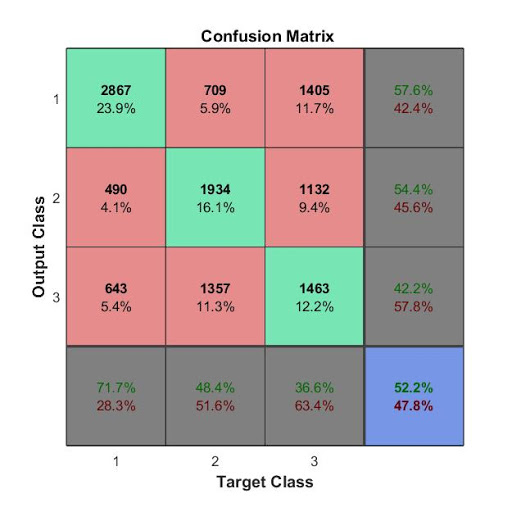
\includegraphics[scale=0.75]{./figuras/confusionmatrix}
%\end{figure}
\subsection{Precis\~ao de classifica\c{c}\~ao}
\par
Precis\~ao de classifica\c{c}\~ao \'e definida como a raz\~ao entre as amostras classificadas corretamente e o numero total de amostras \cite{RAO}.
\begin{equation}\label{eq:ACC}
ACC=\frac{TP+TN}{TP+FN+FP+TN}
\end{equation}
\subsection{Coefficiente Kappa}
Uma outra medida de performance \'e o coeficiente kappa de Cohen:
\begin{equation}\label{eq:kappa}
\kappa=\frac{ACC-ACC_0}{1-ACC_0}
\end{equation}
Onde $ACC$ \'e a precis\~ao de classifica\c{c}\~ao e $ACC_0$ \'e a probabilidade do classificador acertar a classe escolhendo uma classe aleat\'oriamente. Isso torna $\kappa$ uma m\'etrica independente do numero de classes e amostras por classe \cite{RAO}. Um $\kappa = 0$ \'e a performance onde a probabilidade de acerto \'e a mesma que a escolha aleat\'oria e $\kappa = 1$ \'e a performance perfeita.

\clearpage
\section{M\'etodos de estimativa de espectro (PSD)}
\par 
\ac{PSD} extraem informa\c{c}\~oes do sinal como um processo estoc\'astico para descrever a distribui\c{c}\~ao de pot\^encia de um sinal no dom\'inio da frequ\^encia \cite{Comparison2008}.
A \ac{PSD} \'e definido como a transformada de Fourier da fun\c{c}\~ao de autocorrela\c{c}\~ao do sinal contanto que o sinal seja estacion\'ario \cite{Comparison2008}.
Na pr\'atica, as caracter\'isticas estat\'isticas do sinal n\~ao s\~ao conhecidas e s\'o podem ser estimadas de uma sequ\^encia de amostras temporais.
\subsection{Periodograma}
A t\'ecnica de estimativa de espectro $\hat{S}(f)$ mais comum \'e multiplica\c{c}\~ao da transformada de Fourier do sinal $x(t)$ pela sua complexa conjugada, escalonando isto pelo numero de pontos amostrados $N$\cite{PMTM}. 
\begin{equation}
\hat{S}(f)= \frac{X(j2\pi f)  X^{*}(j2\pi f)}{N}
\end{equation}
\begin{equation}\label{eq:winPSD}	
\hat{S}(f)= {\left| \sum_{t=0}^{N-1} x(t) a(t) e^{-2\pi j f t }\right|}^{2} 
\end{equation}
Quando a janela $a(t)$ \'e igual a $1$ ela \'e chamada de janela retangular e esta estimativa \'e chamada de\textbf{ periodograma} \cite{PMTM}.
\par
A confiabilidade da estimativa \'e significativamente reduzida quando h\'a vari\^ancia da estimativa do espectro em cada frequ\^encia $f$ e quando h\'a vazamento de energia em todas frequencias criando um bias\cite{PMTM}.
A vazamento \'e devido ao fato de que utilizamos uma se\c{c}\~ao do sinal que \'e o equivalente a utilizar uma janela retangular.
\cite{PMTM}.
Uma solu\c{c}\~ao a este problema \'e mutiplicar o sinal no dom\'inio do tempo por uma janela n\~ao retangular com uma menor amplitude nas extremidades \cite{PMTM}.
\subsection{Espectro de Welch (PWelch)}
\begin{figure}[!htp]
	\begin{center}
		\caption{Espectro de Welch}
		\scalebox{.8}{
		\tikzstyle{sample}=[minimum height=1cm,minimum width=4cm,xshift=2cm,draw=black]
\tikzstyle{plotsf}=[smooth,yscale=0.05,xscale=8,color=blue]
%\tikzstyle{lines}=[color=black,line width=0.5mm]
\tikzstyle{lines}=[color=black,very thick]
\begin{tikzpicture}[
 brc/.style args = {#1/#2}{decorate,
	decoration={brace, amplitude=5pt,
		raise=#1,#2},% for mirroring of brace
	thick},]
%\begin{axis}[axis line style={draw=none},
%tick style={draw=none},]
%	\addplot table[y=y,x=t,col sep=comma] {./dados/EEG2.csv};
%\end{axis}
\draw (0,0)  [plotsf] plot file {./dados/EEG2.table};
%\draw [thick,double,->] (4.5cm,-3cm)--(4.5cm,-4cm)--(10cm,-4cm) node [midway,below]{\tiny{\textbf{Extra\c{c}\~ao de caracter\'isticas}}};
\draw (0,0) node (s0) [sample,minimum width=16cm,xshift=6cm]{};
\draw [lines, dashdotted ](5.5cm,0.5cm)--(5.5cm,-.5cm);
\draw [lines, dashdotted ](11cm,0.5cm)--(11cm,-0.5cm);
%---------------------------
%Setas para as Janelas FFT
\draw [-latex,very thick](3cm,-0.5cm)--(3cm,-1.8cm)  node[midway,left]{$\hat{S}_1(f)$};
\draw [-latex,very thick](8.5cm,-0.5cm)--(8.5cm,-1.8cm)  node[midway,left]{$\hat{S}_2(f)$};
\draw [-latex,very thick](14cm,-0.5cm)--(14cm,-1.8cm)  node[midway,left]{$\hat{S}_k(f)$};
%---------------------------
%Graficos FFT Janelas
%1
\begin{scope}[xshift=1cm,yshift=-5cm,xscale=-.03,yscale=-.014,rotate=180]%,xcomb]
\draw (-5,0) [color=black,thick]rectangle (125,230);
\draw (0,0)[color=blue,thick]  plot  file {./dados/Welch/W1.table};
\end{scope}
%2
\begin{scope}[xshift=6.5cm,yshift=-5cm,xscale=-.03,yscale=-.014,rotate=180]%,xcomb]
\draw (-5,0) [color=black,thick]rectangle (125,230);
\draw (0,0)[color=blue,thick]  plot  file {./dados/Welch/W2.table};
\end{scope}
%3
\begin{scope}[xshift=12cm,yshift=-5cm,xscale=-.03,yscale=-.014,rotate=180]%,xcomb]
\draw (-5,0) [color=black,thick]rectangle (125,230);
\draw (0,0)[color=blue,thick]  plot  file {./dados/Welch/W3.table};
\end{scope}
%---------------------------
%Espectro de Welch

\begin{scope}[xshift=6.5cm,yshift=-10.5cm,xscale=-.03,yscale=-.014,rotate=180]%,xcomb]
\draw (-5,0) [color=black,thick]rectangle (125,230);
\draw (0,0)[color=blue,thick]  plot  file {./dados/Welch/WMean.table};
\end{scope}
%---------------------------
%SUM
\begin{scope}[xshift=8.3cm,yshift=-6cm]
\node[circle,thick,draw=black] (0,0) {\huge{$+$}};
\end{scope}
%SUM ARROWS
\draw [-latex,very thick](3cm,-5cm)--(3cm,-6cm)--(7.9cm,-6cm);
\draw [-latex,very thick](8.3cm,-5cm)--(8.3cm,-5.5cm);
\draw [-latex,very thick](14cm,-5cm)--(14cm,-6cm)--(8.7cm,-6cm);
%MEAN ARROW
\draw [-latex,very thick](8.3cm,-6.35cm)--(8.3cm,-7.25cm) node[midway,left]{$\frac{1}{K}$};


\end{tikzpicture}
		}
		
		\label{fig:Welch}
	\end{center}	
\end{figure}
O \ac{PWelch}, tamb\'em conhecido como m\'etodo da m\'edia do periodograma consiste em dividir o sinal $x(t)$ em K segmentos $x_k(t)$ parcialmente sobrepostos e calcular a m\'edia do periodograma dos segmentos  \cite{PWelch}.
\begin{equation}
\hat{S}(f)= \frac{1}{K} \sum_{k=1}^{K} \hat{S}_k(f)
\end{equation}
Os passos desse algoritmo podem ser descritos assim:
\pagebreak
\begin{enumerate}
	\item divida o sinal 
	\begin{equation*}
	x[0],x[1],\ldots,X[N-1]
	\end{equation*}
	em $K$ segmentos de comprimento $M$:
	\begin{equation*}
	\begin{aligned}
	\text{Segmento 1: } &x[0],x[1],\ldots,x[M-1]\\
	\text{Segmento 2: } & x[S],x[S+1],\ldots,x[M+S-1]\\
	\vdots & \\
	\text{Segmento K: } & x[N-M],x[N-M+1],\ldots,x[N-1]\\
	\text{onde} &\\
	&M= \text{N\'umero de pontos em cada segmento}\\
	&S= \text{O deslocamento entre os segmentos}\\
	&K = \text{N\'umero de segmentos} \\
	\end{aligned}
	\end{equation*}
	\item Para cada segmento, calcule a \ac{DFT} a uma frequ\^encia $\nu=i/M$:
	\begin{equation*}
	\begin{aligned}
	X_k(\nu)= \sum_m x[m]w[m]e^{-j\pi \ni m}\\
	\text{onde}\\
	m=(k-1)S,\ldots,M+(k-1)S-1\\
	w[m]= a janela\\
	\end{aligned}
	\end{equation*}
	\item Para cada segmento, calcule o valor do periodograma, $P_k(f)$, da transformada de fourier:
	\begin{equation*}
	\begin{aligned}
	P_k(\nu) = \frac{1}{W} {\left| X_k (\nu) \right|}^{2}\\
	onde\\
	W= \sum_{m=0}^{M} w^2 [m]\\  
	\end{aligned}
	\end{equation*}
	\item Calcule a m\'edia dos periodogramas para obter a estimativa de Welch:
	\begin{equation*}
	S_x(\nu)=\frac{1}{K} \sum_{k=1}^{K} P_k(\nu)
	\end{equation*}
\end{enumerate}


\subsection{\textit{Multitaper Power Spectral density} (PMTM)}
\begin{figure}[!htp]
	\begin{center}
		\caption{Multitaper}
		\scalebox{.70}{
		\tikzstyle{sample}=[minimum height=1cm,minimum width=4cm,xshift=2cm,draw=black]
\tikzstyle{plotsf}=[smooth,yscale=0.05,xscale=8,color=blue,]
\tikzstyle{lines}=[color=black,very thick]
\begin{tikzpicture}[
 brc/.style args = {#1/#2}{decorate,
	decoration={brace, amplitude=5pt,
		raise=#1,#2},% for mirroring of brace
	thick},]
	

\begin{scope}[xscale=0.7,yscale=.3]
\begin{axis}[%axis line style={draw=none},
tick style={draw=blue}, yticklabels={,,}, xticklabels={,,},mark repeat=50,ticks=none
]
	\addplot[color=blue] table[y=EEG,x=t,col sep=comma] {./dados/Multitaper/multitaper_all.csv};
\end{axis}
\end{scope}
%----------------------------Tapered EEG--------------
%1
\begin{scope}[xscale=0.7,yscale=.3,yshift=7cm,xshift=8cm]
\begin{axis}[%axis line style={draw=none},
tick style={draw=blue}, yticklabels={,,}, xticklabels={,,},mark repeat=50,ticks=none
]
	\addplot[color=red,loosely dashdotted,very thick] table[y=S1,x=t,col sep=comma] {./dados/Multitaper/multitaper_all.csv};
	\addplot[color=blue] table[y=ES1,x=t,col sep=comma] {./dados/Multitaper/multitaper_all.csv};
\end{axis}
\end{scope}
%2
\begin{scope}[xscale=0.7,yscale=.3,xshift=8cm]
\begin{axis}[%axis line style={draw=none},
tick style={draw=blue}, yticklabels={,,}, xticklabels={,,},mark repeat=50,ticks=none
]
	\addplot[color=red,loosely dashdotted,very thick] table[y=S2,x=t,col sep=comma] {./dados/Multitaper/multitaper_all.csv};
	\addplot[color=blue] table[y=ES2,x=t,col sep=comma] {./dados/Multitaper/multitaper_all.csv};
\end{axis}
\end{scope}
%3
\begin{scope}[xscale=0.7,yscale=.3,yshift=-7cm,xshift=8cm]
\begin{axis}[%axis line style={draw=none},
tick style={draw=blue}, yticklabels={,,}, xticklabels={,,},mark repeat=50,ticks=none
]
	\addplot[color=red,loosely dashdotted,very thick] table[y=S3,x=t,col sep=comma] {./dados/Multitaper/multitaper_all.csv};
	\addplot[color=blue] table[y=ES3,x=t,col sep=comma] {./dados/Multitaper/multitaper_all.csv};
\end{axis}
\end{scope}
%---------------------------Tapered PSDs--------------------
%1
\begin{scope}[xscale=0.55,yscale=.3,yshift=7cm,xshift=21cm]
\begin{axis}[%axis line style={draw=none},
tick style={draw=blue}, yticklabels={,,}, xticklabels={,,},mark repeat=50,ticks=none
]
	\addplot[color=blue] table[y=TS1,x=f,col sep=comma] {./dados/Multitaper/multitaper_all.csv};
\end{axis}
\end{scope}
%2
\begin{scope}[xscale=0.55,yscale=.3,xshift=21cm]
\begin{axis}[%axis line style={draw=none},
tick style={draw=blue}, yticklabels={,,}, xticklabels={,,},mark repeat=50,ticks=none
]
	\addplot[color=blue] table[y=TS2,x=f,col sep=comma] {./dados/Multitaper/multitaper_all.csv};
\end{axis}
\end{scope}
%3
\begin{scope}[xscale=0.55,yscale=.3,yshift=-7cm,xshift=21cm]
\begin{axis}[%axis line style={draw=none},
tick style={draw=blue}, yticklabels={,,}, xticklabels={,,},mark repeat=50,ticks=none
]
	\addplot[color=blue] table[y=TS3,x=f,col sep=comma] {./dados/Multitaper/multitaper_all.csv};
\end{axis}
\end{scope}
%---------------------------------Multitaper---------
\begin{scope}[xscale=0.55,yscale=.3,xshift=32cm]
\begin{axis}[%axis line style={draw=none},
tick style={draw=blue}, yticklabels={,,}, xticklabels={,,},mark repeat=50,ticks=none
]
	\addplot[color=blue] table[y=PSD,x=f,col sep=comma] {./dados/Multitaper/multitaper_all.csv};
\end{axis}
\end{scope}
%-----------------Sum-------------------------
\begin{scope}[xshift=16.5cm,yshift=.8cm]
\node[circle,thick,draw=black] (0,0) {\huge{$+$}};
\end{scope}
%-----------------Arrows----------------------
%-------EEG To Tapered-------
%1
\draw [-latex,very thick](3cm,1.7cm)--(3cm,3cm)--(5.6cm,3cm) node[midway,above]{$\times T_1$};
%2
\draw [-latex,very thick](4.8cm,.8cm)--(5.6cm,.8cm) node[midway,above]{$\times T_2$};
%3
\draw [-latex,very thick](3cm,0cm)--(3cm,-1.4cm)--(5.6cm,-1.4cm) node[midway,above]{$\times T_k$};
%--------Tapered To PSDs------
%1
\draw [-latex,very thick](10.4cm,3cm)--(11.6cm,3cm) node[midway,above]{$\hat{S}_1(f)$};

%2
\draw [-latex,very thick](10.4cm,.8cm)--(11.6cm,.8cm) node[midway,above]{$\hat{S}_2(f)$};

%3
\draw [-latex,very thick](10.4cm,-1.4cm)--(11.6cm,-1.4cm) node[midway,above]{$\hat{S}_k(f)$};
%--------PSDS to Sum-----------
%1
\draw [-latex,very thick](15.3cm,3cm)--(16.5cm,3cm) --(16.5cm,1.2cm) ;

%2
\draw [-latex,very thick](15.3cm,.8cm)--(16.1cm,.8cm) ;

%3
\draw [-latex,very thick](15.3cm,-1.4cm)--(16.5cm,-1.4cm) --(16.5cm,.3cm) ;
%----------Average----------
\draw [-latex,very thick](16.9cm,.8cm)--(17.6cm,.8cm) node[midway,above]{$\frac{1}{K}$};
\end{tikzpicture}
		}

		\label{fig:multitaper}
	\end{center}	
\end{figure}
\par 
\ac{PMTM}, inicialmente descrito por Thomson em 1982, melhora a estimativa espectral ao analisar tanto a vazamento quanto a vari\^ancia na estimativa \cite{PMTM}.
Nesta abordagem, cada janela $v_k$ de um conjunto $K$ de janelas seja ligeiramente diferente e reduza a vazamento de energia em v\'arias frequ\^encias \cite{PMTM}. 
Al\'em disto, as janelas s\~ao ortogonais e s\~ao usadas pra providenciar $K$ amostras ortogonais do sinal $x(t)$.
Estas amostras s\~ao usadas para criar um conjunto de $K$ estimativas $\hat{S}_k (f) $ que podem ser utilizadas para calcular uma  m\'edia $\bar{S}(f)$ com vari\^ancia reduzida \cite{PMTM}.
\begin{equation}
\bar{S}(f) = \frac{1}{K} \sum_{k=1}^{K} \hat{S}_k (f)
\end{equation}
De maneira geral, a aplica\c{c}\~ao de uma janela segue o seguinte padr\~ao: 
Cada janela $a(t)$ \'e associada com uma estimativa de espectro dado pela equa\c{c}\~ao \ref{eq:winPSD} \cite{PMTM}.
Para manter os valores de pot\^encia totais corretos, n\'os assumimos que as janelas s\~ao normalizadas de tal forma que $\sum_{t=0}^{N-1} {\left|  a(t)\right|}^{2}=1 $ \cite{PMTM}. 
Al\'em disso, a pot\^encia do espectro de uma janela $a(t)$ $\left| {A(f)}^{2} \right| $ e suas propriedades s\~ao importantes porque elas determinam, atrav\'es da convolu\c{c}\~ao, a estimativa do nosso espectro do sinal $x(t)$ janelado \cite{PMTM}.
\begin{equation}
\hat{S}(f) = \int_{\frac{-1}{2}}^{\frac{1}{2}} {A(f')}^{2}S(f - f')df'
\end{equation}

\par
Suponha que queremos estimar o nosso espectro com uma banda de resolu\c{c}\~ao $W$, que necessariamente configura um valor entre a resolu\c{c}\~ao do espectro $1/N$ e a frequ\^encia de Nyquist \cite{PMTM}.
Para simplificar a nota\c{c}\~ao assumimos que as amostras entre a unidade e a frequ\^encia de seja normalizado em $\frac{1}{2}$. A fra\c{c}\~ao $\lambda$ da energia da janela dentro da banda selecionada \'e dada por\cite{PMTM}:
\begin{equation}\label{eq:Taper}
\lambda(N,W)=\frac{\int_{-W}^{W}{\left| A(f) \right|}^2 df}{\int_{\frac{1}{2}}^{\frac{1}{2}}{\left| A(f) \right|}^2 df}
\end{equation}

A ideia b\'asicamente \'e de que queremos encontrar as janelas com o m\'inimo de vazamento ao maximizar $\lambda$ a fra\c{c}\~ao de energia dentro da banda $W$ \'e maximizada \cite{PMTM}.
Em suma, $\lambda$ \'e maximizado ao configurar a derivada da express\~ao da equa\c{c}\~ao \ref{eq:Taper} com o vetor $a(t)$ igual a zero \cite{PMTM}.
Isto \'e o equivalente a encontrar os auto valores de uma matriz $N\cross N$ $D$ com os componentes $D_{t,t'}=\frac{2\pi W(t-t')}{\pi(t-t')}$ \cite{PMTM}.
Note de que esta fun\c{c}\~ao \'e sim\'etrica portanto $D$ \'e uma matriz sim\'etrica.
\begin{equation*}
D \cdot \textbf{a} = \lambda \textbf{a}
\end{equation*}
A solu\c{c}\~ao  tem $N$ autovalores $\lambda_k$ e autovetores ($\nu_{1},\nu_{2},\ldots,\nu_{N-1}$) ortonormais  \cite{PMTM}.
O primeiro conjunto de componentes da matriz capturam a maioria das propriedades dessa janela ideal, enquanto os componentes seguintes capturam menos, a quest\~ao \'e quais componentes incluir quando se utiliza eles como janelas\cite{PMTM}. O primeiro autovalor \'e  pr\'oximo de um, portanto ele est\'a associado a um excelente autovetor, em outras palavras uma janela que minimiza o vazamento \cite{PMTM}.
\chapter{Desenvolvimento} \label{lab_desenvolvimento}

%\section{Introdução}
\section{Amostras}
\par
As amostras utilizadas neste trabalho foram obtidas do BCI Competition IV - Graz data set 2B e de acordo com \cite{GrazBData}
 ele se consiste em dados de \ac{EEG} de 9 sujeitos em um estudo.
 Para cada um dos sujeitos 5 sess\~oes foram gravadas em quais primeiras duas sess\~oes contem dados sem feedback (screening), e as ultimas tr\^es sess\~oes foram gravadas com feedback. Nestas sess\~oes os sujeitos tiveram que executar uma imagina\c{c}\~ao motora de duas categorias diferentes (esquerda ou direita) dependendo de uma deixa. 
 \begin{figure}[h!]
 	\caption{segmento EOG nas sess\~oes do graz-b} 	
 	\centering
 	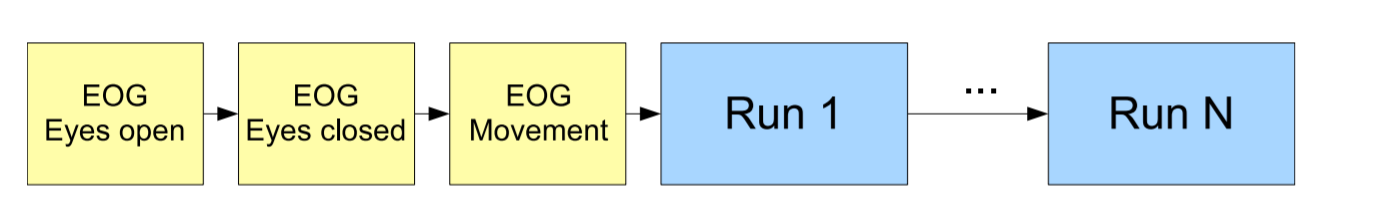
\includegraphics[scale=0.5]{./figuras/graz-eog}
 	\label{fig:Graz-EOG}
 \end{figure}
 \par 
 Os primeiros 5 minutos de cada sess\~ao foram gravados para estimar o efeito do \ac{EOG} no sinal \ac{EEG}.
 Este per\'iodo de grava\c{c}\~ao foi divido em 3 blocos: (1) dois minutos com os olhos abertos (olhando num marcador fixo) (2) um minuto com os olhos fechados e (3) um minuto com os olhos em movimento.
 Este bloco de \ac{EOG} n\~ao est\'a dispon\'ivel para as sess\~oes   B0102T e B0504E, de acordo com a fonte, devido a problemas t\'ecnicos.
 \par
  No processo de grava\c{c}\~ao foram utilizados 3 canais bipolares (C3,Cz e C4) com uma frequ\^encia de amostragem de 250Hz.
 As grava\c{c}\~oes t\'em faixa din\^amica de $\pm 100 \mu$V para as sess\~oes sem feedback e $\pm 50 \mu$V para as sess\~oes com feedback. Elas foram filtrados com um passa-faixa de 0.5Hz a 100Hz e um filtro notch em 50Hz (para reduzir o ru\'ido da rede el\'etrica). O posicionamento para cada um dos eletrodos variou ligeiramente em cada um dos sujeitos.
 Tamb\'em foi gravado o \ac{EOG} com tr\^es eletrodos monopolares usando a mesmas configura\c{c}\~oes de amplica\c{c}\~ao mas com uma faixa din\^amica maior de $\pm 1$mV.
 \par
  \begin{figure}[h!]
 	\caption{Os dois tipos de sess\~ao em Graz-b \cite{GrazBData}. }  	
  	\centering
 	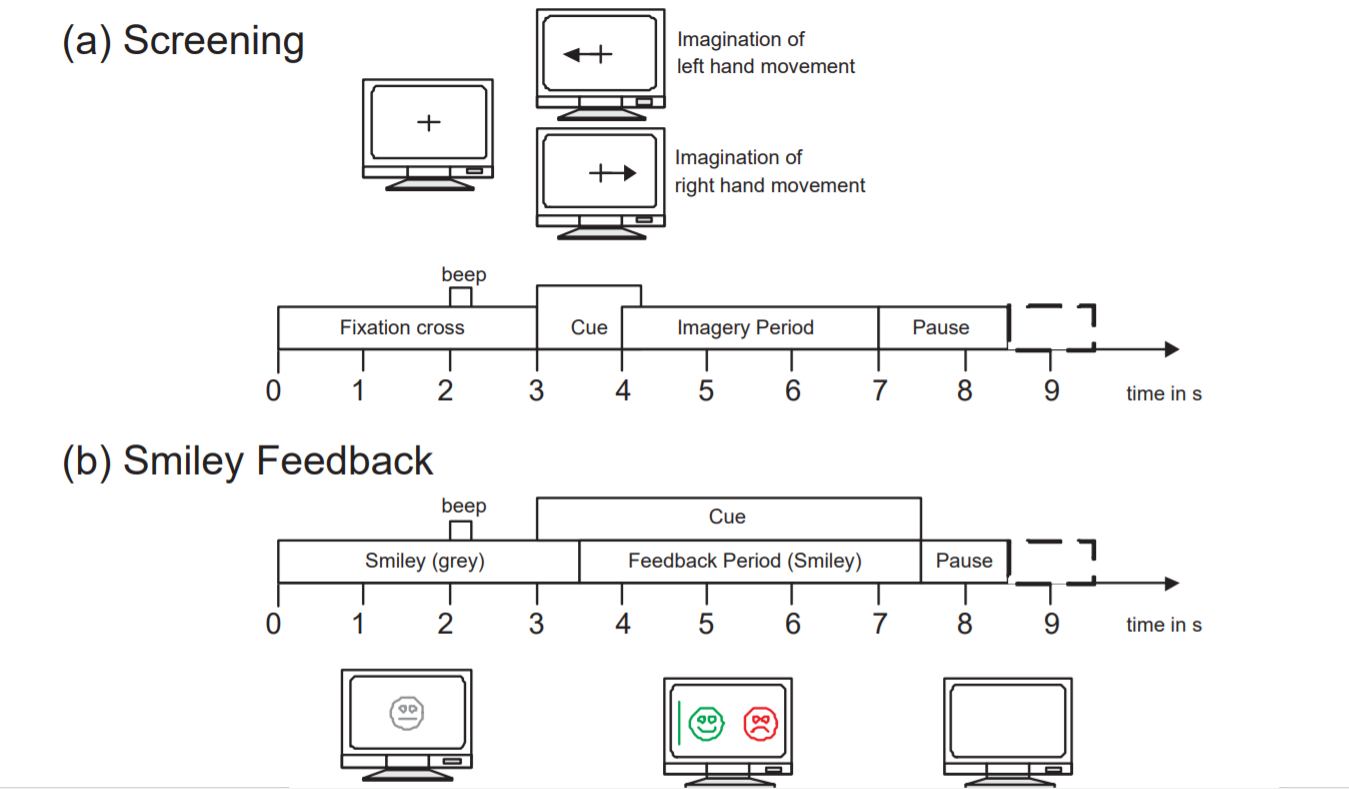
\includegraphics[scale=0.5]{./figuras/graz_b_session}
 	\label{fig:Graz-Session}
 \end{figure}
 As sess\~oes podem divididas em dois tipos
\begin{enumerate}[label=(\alph*)]
	\item \textbf{Sess\~oes sem feedback}: 
	Estas sess\~oes consistem em 6 s\'eries contendo 10 experimentos de cada uma das duas categorias, dando um total de 120 experimentos.
	Neste experimento, nos primeiros 3 segundos foi exibido uma cruz de fixa\c{c}\~ao com um curto aviso sonoro.
	Depois disso uma seta apontando para direita ou esquerda (dependendo do tipo de a\c{c}\~ao motora imagin\'aria) foi utilizado como deixa durando 1.25s .
	 Posteriormente o sujeito teve um período de 4 segundos para imaginar o movimento da m\~ao correspondente ao lado da seta.
	 Para finalizar cada experimento foi seguido por uma parada aleat\'oria de 1.5 a 2.5 segundos para evitar de que o sujeito se adapte.
	\item \textbf{Sess\~oes com feedback}:
	Estas sess\~oes consistiram em 4 s\'eries de 20 experimentos para cada tipo de imagina\c{c}\~ao motora dando um total de 160 experimentos. 
	No inicio deste tipo de sess\~ao foi centralizado um smiley cinza na tela e no segundo posterior foi acionado um aviso sonoro. Ap\'os mais um segundo a deixa foi apresentada dependendo da deixa os sujeitos foram pedidos para moverem o smiley para a direita ou esquerda dando um per\'iodo de 4.5 segundos para imaginar esta a\c{c}\~ao. Caso o smiley fosse movido para o lado correto ele ficaria verde caso contrario vermelho.
	Depois disso, um periodo alet\'orio de 1-2 segundos foi adicionado a cada experimento.
\end{enumerate}
\clearpage
\section{Framework}
\par
Para fazer a compara\c{c}\~ao entre as metodologias  de extra\c{c}\~ao de caracter\'istica e classificadores foi desenvolvido um \textit{framework} para automatizar o processo de treinamento e compara\c{c}\~ao. Este \textit{framework} foi projetado com programa\c{c}\~ao \ac{OOP} em mente devido \`a sua modularidade e f\'acil expans\~ao.
\subsection{Compare Methods}
A fun\c{c}\~ao \textit{CompareMethods} compara todas as configura\c{c}\~oes fornecidas, gera uma tabela com as configura\c{c}\~oes e retorna os classificadores treinados.
\begin{figure}[h!]
	\caption{diagrama compare methods}	
	\centering
	\tikzstyle{block} = [
		% The shape:
		rectangle split,
		rectangle split parts =1,
		% The size:
		minimum size=6mm,
		draw,
		text badly centered,
		draw=blue!80!black!40,
		text=black,
	]
\tikzstyle{decision} = [
		diamond,
		draw,
		text badly centered,
		color=blue,
		aspect=2,
		inner sep=1.5pt,
		scale=0.7,
]
\tikzstyle{begin} = [
		rounded rectangle,
		draw,
		text badly centered,
		minimum size = 1cm,
		color=blue,
]
\tikzstyle{input} = [
ellipse,
draw,
text badly centered,
minimum size = 1cm,
color=blue,
]
\tikzstyle{coord} = [
-stealth,
inner sep =0 pt,
]
\begin{tikzpicture}[node distance= 0.6cm,
transition/.style={very thick,->}
]

\node [begin] (start) {\textbf{In\'icio itera\c{c}\~ao}};
\node[block,rectangle split parts=2] (Sujeito) [below=of start] {\nodepart{one}Sele\c{c}\~ao
	 \nodepart{two} Sujeito};
\node[block,rectangle split parts=2] (DB) [below=of Sujeito]{\nodepart{one}Obten\c{c}\~ao \nodepart{two} Database};
\node[block,rectangle split parts=2] (Dataset) [below=of DB] {\nodepart{one} Obten\c{c}\~ao
\nodepart{two} Dataset};
\node[block,rectangle split parts=1](Train) [below=of Dataset]{
	\nodepart{one} Treinamento classificador
};
\node[block,rectangle split parts=1] (Avaliacao1) [below=of Train]{Avalia\c{c}\~ao performance por Janela amostrada};
%\node []
\draw [transition] (start) -> (Sujeito);
\draw [transition] (Sujeito) -> (DB);
\draw [transition] (DB) -> (Dataset);
\draw [transition] (Dataset) -> (Train);
\draw [transition] (Train) -> (Avaliacao1);
\end{tikzpicture}
	\label{fig:comparemethods}
\end{figure}
\subsection{Trials}
\begin{figure}[h!]
	\caption{diagrama do Trials}	
	\centering
	\tikzstyle{class} = [rectangle split,rectangle split parts=1,draw ,text badly centered, node distance=1cm,scale=0.9]
\begin{tikzpicture}
[edge from parent fork down,sibling distance=4cm,level distance=7cm,
edge from parent/.style={draw,<-,line width=1.2pt}]
\node[class,rectangle split parts=2](Database)
	{
	\nodepart{one}  \textcolor{blue}{\large{Trials}}
	 \nodepart{two} \begin{tabular}{cc}
					\textcolor{purple}{Trials}(path)\\
					\textcolor{purple}{Trials}(path,labels)\\
					\end{tabular}
				
};
\end{tikzpicture}
	\label{fig:Trials}
\end{figure}
%\begin{table}[h!]
%	\centering
%	\caption{M\'etodos da classe Trials}
%	\begin{tabularx}{\textwidth}{c|X}
%		
%		\hline\hline
%		METODO & DESCRI\c{C}\~AO \\ \hline 
%		\textcolor{purple}{Trials} &  \\ \hline
%	\end{tabularx}
%	\label{Tab:metodostrials}
%\end{table}
\textbf{Trials} durante a cria\c{c}\~ao pega o arquivo contendo a sess\~ao de \ac{EEG} filtra os canais de artefatos \ac{EOG} nos canais \ac{EEG} (C3,Cz,C4) usando a \textit{regress\~ao linear} de \cite{EOG2006}, posteriormente ele extrai os experimentos e associa a categoria de imagina\c{c}\~ao motora (1) esquerda e (2) direita ao experimento. Essa informac\~ao \'e obtida do arquivo da sess\~ao ou \'e fornecida atrav\'ez do argumento \textit{labels}.
%\clearpage
\subsection{Database}
\par O \textbf{Database} \'e a classe respons\'avel por fazer a amostragem, extra\c{c}\~ao de caracter\'isticas e de maneira geral preparar os dados para serem utilizados por um classificador. O processo de prepara\c{c}\~ao dos dados para treinamento e valida\c{c}\~ao \'e o seguinte (figura \ref{fig:processoamostragem})
\begin{enumerate}
	\item Durante cria\c{c}\~ao do objeto do tipo \textbf{Database}, cada experimento  armazenado em \textit{Trials} \'e dividido em v\'arias janelas de amostragem com dura\c{c}\~ao $windowLength$ e cada janela tem uma porcentagem de sobreposi\c{c}\~ao com a janela anterior determinada por $overlap$.
	\item As janelas de amostragem s\~ao armazenadas junto com as classifica\c{c}\~oes obtidas do objeto Trials.
	\item \'E gerado um vetor contendo os ind\'ices de amostras aleat\'orias contendo um n\'umero igual de amostras para cada categoria.
	\item De cada janela de amostragem s\~ao extra\'ido os vetores de caracter\'isticas usando a fun\c{c}\~ao de extra\c{c}\~ao de caracter\'isticas configurada. \'E retornado uma matriz contendo o Dataset seguindo o padr\~ao em que os vetores de caracter\'isticas est\~ao nas linhas e na \'ultima coluna consta a categoria da amostra.
\end{enumerate}
\begin{equation}
\left[
\begin{array}{cccc}
F(C3_1) &  F(Cz_1) & F(C4_1) & Cat_1\\ 
F(C3_2) &  F(Cz_2) & F(C4_2) & Cat_2\\ 
\vdots & \vdots & \vdots &\vdots \\
F(C3_n) &  F(Cz_n) & F(C4_n) & Cat_n\\ 
\end{array}
\right]
\end{equation}

\begin{figure}[h!]
	\caption{Amostragem e extra\c{c}\~ao de caracter\'itsticas}	
	\centering
	\tikzstyle{sample}=[minimum height=1cm,minimum width=4cm,xshift=2cm,draw=black]
\tikzstyle{plotsf}=[smooth,yscale=0.05,xscale=8,color=blue]
%\tikzstyle{lines}=[color=black,line width=0.5mm]
\tikzstyle{lines}=[color=black,very thick]
\begin{tikzpicture}[
 brc/.style args = {#1/#2}{decorate,
	decoration={brace, amplitude=5pt,
		raise=#1,#2},% for mirroring of brace
	thick},]
%\begin{axis}[axis line style={draw=none},
%tick style={draw=none},]
%	\addplot table[y=y,x=t,col sep=comma] {./dados/EEG2.csv};
%\end{axis}
\draw (0,0)  [plotsf] plot file {./dados/EEG2.table};
\draw [lines, dashdotted ](2cm,0.5cm)--(2cm,-4cm);
\draw [lines, dashdotted ](4cm,0.5cm)--(4cm,-4cm);
\draw [lines](2cm,-3.5cm)--(4cm,-3.5cm) node [midway,below] {\textbf{overlap}};
\draw [thick,double,->] (4.5cm,-3cm)--(4.5cm,-4cm)--(10cm,-4cm) node [midway,below]{\tiny{\textbf{Extra\c{c}\~ao de caracter\'isticas}}};
\draw (0,0) node (s0) [sample,minimum width=16cm,xshift=6cm]{};
\begin{scope}[yshift=-1.25cm]
\draw (0,0) [plotsf] plot file {./dados/EEG1-1.table};
\draw (0,0) node (s1) [sample] {};
\end{scope}
\node (s1text) [right=of s1,xshift=-1cm]{Janela 1};
\begin{scope}[yshift=-2.5cm]
\draw (0,0)[plotsf] plot  file {./dados/EEG1-2.table};
\draw (0,0) node (s2) [sample,xshift=2cm] {};
\end{scope}
\node (s1text) [right=of s2,xshift=-1cm]{Janela 2};
\begin{scope}[xshift=10cm,yshift=-5cm]
\begin{scope}[scale=0.6]
\begin{axis}[%axis line style={draw=none},
tick style={draw=none},
]
	\addplot table[y=P,x=f,col sep=comma] {./dados/EEGWelch2.csv};
\end{axis}
\end{scope}
\end{scope}
\draw[brc=2mm/](0,0.5)--(16,0.5) node [midway,above,yshift=6]{\textbf{Experimento}};
\end{tikzpicture}
	\label{fig:processoamostragem}
\end{figure}
\begin{figure}[h!]
	\caption{diagrama do Database}	
	\centering
	\tikzstyle{class} = [rectangle split,rectangle split parts=1,draw ,text badly centered, node distance=1cm,scale=0.9]
\begin{tikzpicture}
[edge from parent fork down,sibling distance=4cm,level distance=7cm,
edge from parent/.style={draw,<-,line width=1.2pt}]
\node[class,rectangle split parts=2](Database)
	{
	\nodepart{one}  \textcolor{blue}{\large{Database}}
	 \nodepart{two} \begin{tabular}{cc}
					\textcolor{purple}{Database}(overlap,windowLength,Trials)\\
					\textcolor{purple}{getSampleCountPerLabel}()\\
					\textcolor{purple}{generateDatasetIndex}(numSamples)\\
					\textcolor{purple}{generateDataset}(TrainingDataset)\\
					\textcolor{purple}{getSample}(Range)\\
					\textcolor{purple}{getSampleCount}()\\
					\textcolor{purple}{setFeatureExtractionFcn}(FEFunction)\\
					\end{tabular}
				
};
\end{tikzpicture}
	\label{fig:Database}
\end{figure}
\begin{table}[h!]
	\centering
	\caption{M\'etodos da classe Database}
	\begin{tabularx}{\textwidth}{c|X}		
		\hline\hline
		METODO & DESCRI\c{C}\~AO \\ \hline 
		\textcolor{purple}{Database} & Cria um objeto da classe Database contendo as amostras do objeto da classe Trials usando os par\^ametros \textit{overlap} e \textit{windowLength} para gerar as amostras. \\ \hline
		\textcolor{purple}{getSampleCountPerLabel} & Retorna a quantidade de janelas de amostragem de cada categoria\\ \hline
		\textcolor{purple}{generateDatasetIndex} &  Gera o \'indice do dataset contendo o n\'umero de janelas de amostragem \textit{numSamples}\\ \hline
		\textcolor{purple}{generateDataset} & Retorna o dataset contendo os vetores de caracter\'isticas seguido pelas suas categorias \\ \hline
		\textcolor{purple}{getSample} & Retorna as janelas de amostragem com o seus \'indices determinado por \textit{Range} \\ \hline
		\textcolor{purple}{getSampleCount} &  Retorna o n\'umero total de janelas de amostragem\\\hline
		\textcolor{purple}{setFeatureExtractionFcn} & Configura a func\~ao de extra\c{c}\~ao de caracter\'isticas \\ \hline
	\end{tabularx}
	\label{Tab:metodosdb}
\end{table}
\clearpage
\subsection{FeatureExtractionFnc}
\'E a classe contendo a fun\c{c}\~ao de extra\c{c}\~ao de caracter\'isticas.A fun\c{c}\~ao \textit{ExtractFeature}, virtual na classe base, foi implementada em tr\^es classes derivadas. S\~ao elas: o \acf{PWelch}, \acf{PMTM} e \ac{PSDp}. Para o \ac{PSDp} e \ac{PWelch} foram utilizadas janelas retangulares. Todas as configura\c{c}\~oes restantes s\~ao as padr\~oes do \textbf{MATLAB™}.
\begin{figure}[h!]
	\caption{diagrama de heran\c{c}a do FeatureExtractionFnc}	
	\centering
	\tikzstyle{class} = [rectangle split,rectangle split parts=1,draw ,text badly centered, node distance=1cm,scale=0.7]
\begin{tikzpicture}
[edge from parent fork down,sibling distance=5cm,level distance=4cm,
edge from parent/.style={draw,<-,line width=1.2pt}]
\node[class,rectangle split parts=2](FeatureExtractionFnc)
	{
	\nodepart{one}  \textcolor{blue}{\large{\textit{FeatureExtractionFnc}}}
	 \nodepart{two} \begin{tabular}{cc}
	 					 \textit{\textcolor{purple}{ExtractFeature}}(C3,Cz,C4)\\
					\end{tabular}
	}
	child{ node [class, rectangle split parts=2] (PWelch)
		{
		\nodepart{one} \large{\textcolor{blue}{PWelch}}
		\nodepart{two} \begin{tabular}{cc}
							\textcolor{purple}{ExtractFeature}(C3,Cz,C4)\\
						\end{tabular}
		}
	}
	child{ node [class, rectangle split parts=2] (PSD)
		{
		\nodepart{one} \large{\textcolor{blue}{PSD}}
		\nodepart{two} \begin{tabular}{cc}
		\textcolor{purple}{ExtractFeatures}(C3,Cz,C4)\\
		\end{tabular}
		}
	}
	child{ node [class, rectangle split parts=2] (PMTM)
		{
		\nodepart{one} \large{\textcolor{blue}{PMTM}}
		\nodepart{two} \begin{tabular}{cc}
		\textcolor{purple}{ExtractFeatures}(C3,Cz,C4)\\
		\end{tabular}
		}
	};
\end{tikzpicture}
	\label{fig:FeatureExtraction}
\end{figure}

\clearpage
\subsection{Classifier}
\begin{figure}[h!]
	\caption{diagrama de heran\c{c}a do Classifier}	
	\centering
	\tikzstyle{class} = [rectangle split,rectangle split parts=1,draw ,text badly centered, node distance=1cm,scale=0.7]
\begin{tikzpicture}
[edge from parent fork down,sibling distance=4cm,level distance=7cm,
edge from parent/.style={draw,<-,line width=1.2pt}]
\node[class,rectangle split parts=3](Classifier)
	{
	\nodepart{one}  \textcolor{blue}{\large{\textit{Classifier}}}
	 \nodepart{two} \begin{tabular}{cc}
	 					 \textit{\textcolor{purple}{train}}()\\
 						 \textit{\textcolor{purple}{predict}}()\\
					\end{tabular}
	 \nodepart{three} \begin{tabular}{cc}
					\textcolor{purple}{calculatePerformance}(ValidationSet)\\
					\textcolor{purple}{exportModel}()\\
					\textcolor{purple}{loadModel}(Model)\\
					\textcolor{purple}{loadTrainingData}(TrainingDataset)\\
					\end{tabular}
				
	}
	child{ node [class, rectangle split parts=2] (LinearSVM)
		{
		\nodepart{one} \large{\textcolor{blue}{LinearSVM}}
		\nodepart{two} \begin{tabular}{cc}
							\textcolor{purple}{LinearSVM}()\\
							\textcolor{purple}{train}()\\
							\textcolor{purple}{predict}()\\
						\end{tabular}
		}
	}
	child{ node [class, rectangle split parts=2] (gaussianSVM)
		{
		\nodepart{one} \large{\textcolor{blue}{gaussianSVM}}
		\nodepart{two} \begin{tabular}{cc}
		\textcolor{purple}{gaussianSVM}(KernelScale)\\
		\textcolor{purple}{train}()\\
		\textcolor{purple}{predict}()\\
		\end{tabular}
		}
	}
	child{ node [class, rectangle split parts=2] (kNN)
		{
		\nodepart{one} \large{\textcolor{blue}{kNN}}
		\nodepart{two} \begin{tabular}{cc}
		\textcolor{purple}{kNN}(numNeighbours)\\
		\textcolor{purple}{train}()\\
		\textcolor{purple}{predict}()\\
		\end{tabular}
		}
	}
	child{ node [class, rectangle split parts=2] (ANN)
		{
			\nodepart{one} \large{\textcolor{blue}{ANN}}
			\nodepart{two} \begin{tabular}{cc}
			\textcolor{purple}{ANN}(Layers)\\
			\textcolor{purple}{train}()\\
			\textcolor{purple}{predict}()\\
			\end{tabular}
		}
};
\end{tikzpicture}
	\label{fig:Classifier}
\end{figure}
\begin{table}[h!]
	\centering
	\caption{M\'etodos da classe Classifier}
	\begin{tabularx}{\textwidth}{c|X}
		
		\hline\hline
		METODO & DESCRI\c{C}\~AO \\ \hline 
		\textcolor{purple}{train} & Treina o classificador  \\ \hline
		\textcolor{purple}{predict} & Determina a classifica\c{c}\~ao dos dados de entrada \\ \hline
		\textcolor{purple}{calculatePerformance} & Aceita o par\^ametro ValidationSet, contendo o conjunto de valida\c{c}\~ao e retorna a performance do classificador em percentual de acertos e $\kappa$ de Cohen. \\ \hline
		\textcolor{purple}{exportModel} & Exporta o modelo do classificador \\ \hline
		\textcolor{purple}{loadTrainingData} & Carrega o conjunto de treinamento TrainingDataset.\\ \hline
	\end{tabularx}
	\label{Tab:metodosclass}
\end{table}
 \textbf{Classifier}  \'e uma classe abstrata que descreve os classificadores e cont\'em os m\'etodos descritos na tabela \ref{Tab:metodosclass}.
Os m\'etodos train e predict s\~ao virtuais na classe base e realizam o treinamento e a classifica\c{c}\~ao dos dados nas seguintes classes derivadas:
%Estas s\~ao \textbf{LinearSVM}, \textbf{gaussianSVM}, \textbf{kNN} e \textbf{ANN} estas classes implementam respectivamente um classificador do tipo \ac{SVM} com kernel linear, um \ac{SVM} com kernel gaussiano, \ac{kNN} e um \ac{ANN}.
\begin{enumerate}
	\item \textbf{LinearSVM} implementa um \ac{SVM} com kernel linear.
	\item \textbf{gaussianSVM} implementa um \ac{SVM} com kernel gaussiano durante a inicializa\c{c}\~ao \'e poss\'ivel especificar o par\^ametro $\gamma$ do kernel usando o argumento KernelScale
	\item \textbf{k-NN} \'e um classificador \acs{kNN} com m\'etrica euclidiana que permite, no seu construtor, a especifica\c{c}\~ao da quantidade de viz\'inhos pr\'oximos ($k$).	  
	\item \textbf{ANN} \'e uma rede neural utilizando-se da fun\c{c}\~ao de ativa\c{c}\~ao do tipo \textit{tanh}, \ac{SCG} como o m\'etodo de treinamento e a entropia cruzada como fun\c{c}\~ao de erro. O n\'umero de neur\^onios e a quantidade de camadas ocultas pode ser passada pelo argumento Layers durante a inicializa\c{c}\~ao (por padr\~ao, os objetos desta classe s\~ao configurados com duas camadas ocultas de 20 neu\^onios cada).
\end{enumerate}
\section{M\'etodos de avalia\c{c}\~ao de performance}
\par 
Foram utilizadas 2 m\'etricas de avalia\c{c}\~ao de performance.
A primeira envolve classificar janelas de amostragem isoladas e calcular o $\kappa$ de Cohen e a preci\c{c}\~ao de classifica\c{c}\~ao.
 Esta m\'etrica foi escolhida para poder analisar o impacto da redu\c{c}\~ao da largura da janela de amostragem.
\par
O segundo m\'etodo consiste em obter todas as janelas de amostragem de um experimento, classificar elas e considerar a classifica\c{c}\~ao do experimento como a moda das janelas de amostragem. Depois disso calculado o $\kappa$ de Cohen e a precis\~ao de classifica\c{c}\~ao do experimento.
 Essa m\'etrica foi usada para comparar a performance destes m\'etodos com os utilizados na competi\c{c}\~ao \ac{BCI}-IV 2008 que utilizou o mesmo dataset.
\chapter{Resultados e An\'alises} \label{lab_Resultados}
\section{Performances M\'edias}
\subsection{Overlap vs Janela de Amostragem}
\par
A figura \ref{fig:kappa-over-vs-win} sugere usar um valor de 25\% de overlap, que produz o melhor resultado entre os valores verificados. Esta observa\c{c}\~ao pode ser explicada com uma semelhan\c{c}a maior entre as observa\c{c}\~oes se as janelas tiverem um overlap de 50\%, o que tem impacto negativo no desempenho do classificador.
Tamb\'em podemos notar que a performance se beneficia de janelas de amostragem maior. Entretanto, esse efeito se reduz a partir de 25\% de overlap e janelas de um segundo.
\begin{figure}[!h]
	\caption{(A) Kappa Overlap vs Window (B) Kappa Overlap vs Window para o experimento completo}
	\label{fig:kappa-over-vs-win}
	\begin{tikzpicture}
\begin{axis}[ybar,
ylabel={\textbf{{\LARGE $\kappa$} - Cohen}},
symbolic x coords={0,25,50},
enlargelimits=0.15,
bar width=7pt,
xlabel=\textbf{{Overlap \%}},
scale=1,
ymin=0.05,
ymax=0.37,
xtick=data,
legend style={at={(0.5,-0.25)},anchor=north,legend columns=-1},
]
\addlegendimage{empty legend}
\addlegendentry[]{\textbf{Janela}  }


\addplot coordinates{
	(0,0.145756921970514)
	(25,0.217953198653199)
	(50,0.222418529316488)
	
};
\addlegendentry{0.5s}
\addplot coordinates {
	(0,0.193445731381201)
	(25,0.295532180595581)
	(50,0.228335707502374)
};
\addlegendentry{1s}
\addplot coordinates {
	(0,0.253022486772487)
	(25,0.305006613756614)
	(50,0.271798941798942)
};
\addlegendentry{2s}

\end{axis}
\node[] at (-1,6) {\textbf{A}};
\end{tikzpicture}
	\begin{tikzpicture}
\begin{axis}[ybar,
ylabel={\textbf{{\LARGE $\kappa$} - Cohen}},
symbolic x coords={0,25,50},
enlargelimits=0.15,
bar width=7pt,
xlabel=\textbf{{Overlap \%}},
scale=1,
ymin=0.05,
ymax=0.37,
xtick=data,
legend style={at={(0.5,-0.25)},anchor=north,legend columns=-1},
]

\addlegendimage{empty legend}
\addlegendentry[]{\textbf{Janela}  }

\addplot coordinates{
	(0,0.194592780487009)
	(25,0.301151008868141)
	(50,0.297452810791095)
	
};
\addlegendentry{0.5s}
\addplot coordinates {
	(0,0.213851347718643)
	(25,0.360070705941324)
	(50,0.288910829755114)
};
\addlegendentry{1s}
\addplot coordinates {
	(0,0.2669239009365)
	(25,0.358554160497779)
	(50,0.299020891771033)
};
\addlegendentry{2s}
\end{axis}
\node[] at (-1,6) {\textbf{B}};
\end{tikzpicture}
\end{figure}
\subsection{Classificadores}
Na figura \ref{fig:ClassPerf} podemos observar que por uma margem significativa o classificador com a melhor performance foi o  \ac{L-SVM}. As redes neurais (\acs{ANN-2} e \acs{ANN-3} tiveram performances medianas junto com o \ac{C-SVM}.
 A pior performance por uma margem significativa foi do \ac{F-SVM} em que o parâmetro $K$ do kernel teve um impacto negativo na generaliza\c{c}\~ao do classificador. 
\begin{figure}[h]
	\caption{Performance m\'edia dos classificadores utilizados}
	\label{fig:ClassPerf}
	\centering
	\begin{tikzpicture}
\begin{axis}[ybar,
ylabel={\textbf{{\LARGE $\kappa$} - Cohen}},
symbolic x coords={ANN-2,ANN-3,F-SVM,C-SVM,L-SVM},
enlargelimits=0.15,
bar width=7pt,
xlabel={\textbf{Classificador}},
xtick=data,
legend style={at={(0.5,-0.2)},anchor=north,legend columns=-1},
scale=1.2,
ymin=0.05,
]
\addplot coordinates {
	(ANN-2,0.256710322461084)
	(ANN-3,0.253969286000733)
	(F-SVM,0.08251886405747)
	(C-SVM,0.265203892414323)
	(L-SVM,0.32674780825939)
};
\addplot coordinates {
	(ANN-2,0.311612621296827)
	(ANN-3,0.304360005958168)
	(F-SVM,0.106615596193986)
	(C-SVM,0.305949166653495)
	(L-SVM,0.405089519212324)
};
\legend{Janela isolada,Experimento}
\end{axis}
\end{tikzpicture}
\end{figure}
\subsection{Fun\c{c}\~oes de extra\c{c}\~ao vs Janela de Amostragem}
A figura \ref{fig:PSDPerf} sugere que com o aumento da janela de amostragem a performance melhora igualmente para os \ac{PWelch} e \ac{PMTM} sendo que o desempenho do \ac{PMTM} foi ligeiramente maior. O \ac{PSDp} teve claramente a pior performance isso \'e poss\'ivelmente devido \`a sua falta de capacidade de lidar com ru\'idos. 
\begin{figure}[h]
	\caption{Performance m\'edia das Fun\c{c}\~oes de extra\c{c}\~ao utilizadas vs Janela de amostragem}
	\label{fig:PSDPerf}
	\centering
	\begin{tikzpicture}
\begin{axis}[ybar,
ylabel={\textbf{{\LARGE $\kappa$} - Cohen}},
symbolic x coords={0.5,1,2},
enlargelimits=0.15,
bar width=7pt,
xlabel={\textbf{Janela de Amostragem (s)}},
xtick=data,
legend style={at={(0.5,-0.2)},anchor=north,legend columns=-1},
scale=1.2,
ymin=0.05,
]

\addplot coordinates {

	(0.5,0.168200019315786)
	(1,0.20381375312512)
	(2,0.212802028218695)

};
\addlegendentry[]{PSDp}
\addplot coordinates {
	(0.5,0.208379846569074)
	(1,0.252435974315611)
	(2,0.298970458553792)
};
\addlegendentry[]{PWelch}
\addplot coordinates {
	(0.5,0.209548784055341)
	(1,0.261063892038425)
	(2,0.318055555555556)
};
\addlegendentry[]{PMTM}
\end{axis}
\end{tikzpicture}
\end{figure}
\section{Melhores Performances}
\par Pode-se observar nas tabelas abaixo a preval\^encia do \ac{L-SVM} nas melhores posi\c{c}\~oes entre os classificadores e do \ac{PMTM} nas fun\c{c}\~oes de extra\c{c}\~aos. Na performance utilizando o intervalo completo e na performance de janela de amostragem de at\'e 2 segundos o melhor overlap foi de 25\% enquanto para a performance de at\'e 0.5 segundos o melhor overlap foi o de 50\%.
\begin{table}[h!]
	\centering
	\caption{Melhores performances na m\'etrica do experimento}
	\begin{tabularx}{\textwidth}{c|c|c|c|c|c|c|c|c}		
		\hline\hline
		Pos&$\kappa_1$ &$\text{ACC}_1$&$\kappa_2$&$\text{ACC}_2$&Janela& Overlap&Fun\c{c}\~ao&Classificador  \\ \hline 
		$1^{\underline{o}}$&0.422&71.14\%&0.526&76.32\%&2s&25\%&PWelch&\acs{L-SVM} \\ \hline 
		$2^{\underline{o}}$&0.426&71.35\%&0.512&75.62\%&2s&25\%&PMTM&L-SVM \\ \hline
		$3^{\underline{o}}$&0.421&71.06\%&0.491&74.58\%&2s&25\%&PMTM&\acs{ANN-3} \\ \hline
		$4^{\underline{o}}$&0.407&70.36\%&0.490&74.51\%&1s&25\%&PMTM&L-SVM \\ \hline
		$5^{\underline{o}}$&0.402&70.11\%&0.484&74.23\%&1s&25\%&PMTM&\ac{ANN-2} \\ \hline
	\end{tabularx}
	\label{Tab:melhoresKappaFull}
\end{table}

\begin{table}[h!]
	\centering
	\caption{Melhores performances por Janela de amostragem de at\'e 2s}
	\begin{tabularx}{\textwidth}{c|c|c|c|c|c|c|c|c}		
		\hline\hline
		Pos&$\kappa_1$ &$\text{ACC}_1$&$\kappa_2$&$\text{ACC}_2$&Janela& Overlap&Fun\c{c}\~ao&Classificador  \\ \hline
		$1^{\underline{o}}$&0.426&71.35\%&0.512&75.62\%&2s&25\%&PMTM&L-SVM \\ \hline 
		$2^{\underline{o}}$&0.422&71.14\%&0.526&76.32\%&2s&25\%&PWelch&L-SVM\\ \hline
		$3^{\underline{o}}$&0.421&71.07\%&0.452&72.61\%&2s&0\%&PMTM&L-SVM \\ \hline
		$4^{\underline{o}}$&0.421&71.06\%&0.491&74.58\%&2s&25\%&PMTM&ANN-3 \\ \hline
		$5^{\underline{o}}$&0.418&70.95\%&0.466&73.33\%&2s&50\%&PMTM&L-SVM \\ \hline
	\end{tabularx}
	\label{Tab:melhoresKappa}
\end{table}

\begin{table}[h!]
	\centering
	\caption{Melhores performances por Janela de amostragem de at\'e 0.5s}
	\begin{tabularx}{\textwidth}{c|c|c|c|c|c|c|c|c}		
		\hline\hline
		Pos&$\kappa_1$ &$\text{ACC}_1$&$\kappa_2$&$\text{ACC}_2$&Janela& Overlap&Fun\c{c}\~ao&Classificador  \\ \hline
		$1^{\underline{o}}$&0.293&64.69\%&0.401&70.09\%&0.5s&	50\%&PMTM&L-SVM \\ \hline 
		$2^{\underline{o}}$&0.286&64.31\%&0.388&69.45\%&0.5s&	50\%&PWelch&L-SVM \\ \hline
		$3^{\underline{o}}$&0.284&64,21\%&0.399&69.98\%&0.5s&25\%&PMTM&L-SVM \\ \hline
		$4^{\underline{o}}$&0.280&64,01\%&0.397&69.88\%&0.5s&25\%&PWelch&L-SVM \\ \hline
		$5^{\underline{o}}$&0.275&63.78\%&0.391&69.57\%&0.5s&	25\%&PMTM&ANN-2 \\ \hline
	\end{tabularx}
	\label{Tab:melhoresKappa125}
\end{table}

\chapter{Conclusão} \label{lab_conclusao}
\par
Em conclus\~ao, o melhor classificador foi o SVM com um kernel linear. O melhor overlap é de 25\% e, dependendo da aplica\c{c}\~ao, qualquer tamanho de janela pode ser utilizado com um pequeno ganho de performance com uma largura de 2s. 
\par
Por fim, a melhor configura\c{c}\~ao utilizada teve uma performance pr\'oxima aos classificadores utilizados durante a competi\c{c}\~ao, apesar de ser claramente inferior \`a primeira posi\c{c}\~ao. 
\begin{table}[h!]
	\centering
	\caption{Resultados da competi\c{c}\~ao BCI-IV 2008}
	\begin{tabularx}{\textwidth}{c|X|c|c|c|c|c|c|c|c|c|c}		
		\hline\hline
		Pos&contributor&$\kappa$&1&2&3&4&5&6&7&8&9  \\ \hline
		$1^{\underline{o}}$&Z. Y. Chin&\textbf{0.60}&0.40&0.21&0.22&	0.95&0.86&0.61&0.56&0.85&0.74 \\ \hline 
		$2^{\underline{o}}$&H. Gan&\textbf{0.58}&0.42&0.21&0.14&0.94&0.71 &0.62&0.61&0.84&0.78 \\ \hline
		$3^{\underline{o}}$&D. Coyle&\textbf{0.46}&0.19&0.12&0.12 &0.77&0.57&0.49&0.38&0.85&0.61 \\ \hline
		$4^{\underline{o}}$&S. Lodder&\textbf{0.43}&0.23&0.31&0.07&0.91& 	0.24&0.42&0.41&0.74&0.53 \\ \hline
		$5^{\underline{o}}$&J. F. D. Saa&\textbf{0.37}&0.20&0.16&0.16&0.73&0.21&0.19&0.39&0.86&0.44 \\ \hline
		$6^{\underline{o}}$&Y. Ping&\textbf{0.25}&0.02&0.09&0.07&0.43&0.25&0.00&0.14&0.76&0.47\\ \hline\hline
		-&L-SVM PMTM&\textbf{0.51}&0.41&0&0.09&0.92&0.58&0.63&0.4&0.83&0.71\\ \hline
	\end{tabularx}
	\label{Tab:BCI2008}
\end{table}

%\section{Trabalhos Futuros}
%\par Ap\'os a conclusão deste TCC foi desenvolvido nova abordagem, utilizando uma combina\c{c}\~ao entre GAN, CNN e SVM que teve um $\kappa$ de $0.4$ para uma janela de 0.5s. Estes algoritmos ainda estão em estado de desenvolvimento e, por este motivo, n\~ao foram inclu\'idos no escopo do presente TCC.




\postextual
%	\bibliographystyle{abnt}
	\bibliography{bibliografia}
%\appendix
%\chapter{Informações Adicionais}

\begin{flushright}
Juiz de Fora, 29 de maio de 2017
\end{flushright}

Prezado(a) aluno(a), 

Esta é a versão 1.4 do \emph{template} elaborado pelos membros da \ac{CTCC}, com a colaboração de professores do curso. As principais modificações em relação à versão anterior são:
\begin{itemize}
	\item Correção no título da seção de ``Abreviaturas e Siglas'';
	\item Modificação do texto de apresentação do trabalho;
	\item Correção das legendas das tabelas (que devem ser posicionadas acima de cada tabela).
\end{itemize}

O contato com a comissão pode ser realizado pelo \emph{e-mail} \textbf{mecatronica.jf@ifsudestemg.edu.br}. O regulamento e os documentos relativos ao \ac{TCC} estão disponíveis no endereço 
\hyperlink{sites.jf.ifsudestemg.edu.br/mecatronica/tcc}{\textbf{sites.jf.ifsudestemg.edu.br/mecatronica/tcc}}.

Desejamos um bom trabalho!

\vspace*{4\baselineskip}
\begin{center}
CTCC - Engenharia Mecatrônica

IF Sudeste MG - \emph{Campus} Juiz de Fora
\end{center}





	
%%---Apêndice	
%\begin{apendicesenv}
%	\chapter{Informações Adicionais}

\begin{flushright}
Juiz de Fora, 29 de maio de 2017
\end{flushright}

Prezado(a) aluno(a), 

Esta é a versão 1.4 do \emph{template} elaborado pelos membros da \ac{CTCC}, com a colaboração de professores do curso. As principais modificações em relação à versão anterior são:
\begin{itemize}
	\item Correção no título da seção de ``Abreviaturas e Siglas'';
	\item Modificação do texto de apresentação do trabalho;
	\item Correção das legendas das tabelas (que devem ser posicionadas acima de cada tabela).
\end{itemize}

O contato com a comissão pode ser realizado pelo \emph{e-mail} \textbf{mecatronica.jf@ifsudestemg.edu.br}. O regulamento e os documentos relativos ao \ac{TCC} estão disponíveis no endereço 
\hyperlink{sites.jf.ifsudestemg.edu.br/mecatronica/tcc}{\textbf{sites.jf.ifsudestemg.edu.br/mecatronica/tcc}}.

Desejamos um bom trabalho!

\vspace*{4\baselineskip}
\begin{center}
CTCC - Engenharia Mecatrônica

IF Sudeste MG - \emph{Campus} Juiz de Fora
\end{center}





%\end{apendicesenv}

\end{document}
